\documentclass[xcolor={x11names,svgnames}]{beamer}

\usepackage[french]{babel}
\usepackage[T1]{fontenc}
\usepackage{cellspace}

\usepackage{amsmath}
\usepackage{amsfonts}
\usepackage{tikz}
\usepackage{xspace}
\usepackage[normalem]{ulem}
\usepackage{minted}

\usepackage{marvosym}
\usepackage{pifont}

\newcommand{\bigO}[1]{\ensuremath{\mathcal{O}\left( #1 \right)} }
\newcommand{\triste}{\includegraphics[width=0.5cm,trim=0 17mm 0 0]{triste}}

\newcommand{\red}{\alert}
\newcommand{\green}{\color{LimeGreen}}
\newcommand{\blue}{\color{cyan}}

% FORTIN
\newcommand{\mynote}[1]{\note<1>[item]{#1}}
\newcommand{\euro}{\EUR\xspace}

\usetikzlibrary{patterns}
\usetikzlibrary{snakes}
 \usetikzlibrary{arrows}
\usetikzlibrary{backgrounds}
\usetikzlibrary{shapes}
\usetikzlibrary{shadows}
\usetikzlibrary{calc}
\usetikzlibrary{decorations}
\usetikzlibrary{decorations.pathmorphing}
\usetikzlibrary{decorations.shapes}
\usetikzlibrary{decorations.markings}
\usetikzlibrary{positioning}

\definecolor{amethyst}{rgb}{0.6, 0.4, 0.8}
\definecolor{cyan}{rgb}{0,0.6796875,1}

\usecolortheme{rose}
\setbeamertemplate{footline}{}
\setbeamertemplate{navigation symbols}{}

\usepackage{fontspec}

\setsansfont{PalatinoSansLTPro}[
   Path = /home/charles/charles_work/fonts/PalatinoSans/, 
   Extension      = .otf,
   UprightFont    = *-Regular,
   BoldFont= *-Bold ,
   ItalicFont = *-Italic,
   BoldItalicFont = *-BoldIta
]

%\author[C.~Bouillaguet]{Charles Bouillaguet \newline
%  {\small (\texttt{charles.bouillaguet@lip6.fr})}}

\title{Cours 1 : Introduction}
%\date{2020-01-27}

\begin{document}

\begin{frame}[fragile]

  Charles Bouillaguet (\verb|charles.bouillaguet@lip6.fr|)
  
  \begin{exampleblock}{Credits}
    \begin{itemize}
    \item Ce cours est basé sur celui de Pierre Fortin (SU $\leadsto$ ULille)
    \item Celui de P. Fortin était basé sur celui de  J.-L. Lamotte (SU)
    \end{itemize}
  \end{exampleblock}

  \begin{block}{Bibliographie}
    \begin{itemize}
    \item {\small \textit{Parallel Programming in C with MPI and OpenMP} (M.J. Quinn)}
    \item \textit{MPI: A Message-Passing Interface Standard}
    \item \textit{OpenMP Application Programming Interface}
    \item ...
    \end{itemize}
  \end{block}


% \item U.C. Berkeley CS267 (J. Demmel,  \url{http://www.cs.berkeley.edu/~demmel} )
%   \item Univ. Tennessee Knoxville CS 594 (J. Dongarra, {\small \url{http://www.netlib.org/utk/people/JackDongarra/courses.htm}})
%   \item Computer Architecture, A Quantitative Approach (J.L. Hennessy \&
%     D.A. Patterson, fifth edition) 
% %  \item Architectures et Systèmes des Calculateurs Parallèles 
% %    (cours de F. Pellegrini, ENSEIRB) 
%   \end{itemize}
  
\end{frame}


%%%%%%%%%%%%%%%%%%%%%%%%%%%%%%%%%%%%%%%%%%%%%%%%%%%%%%%%%%%%%%%%%%%%%

\section{Introduction blabla}

\begin{frame}[label=title]
  \titlepage
\end{frame}
 
 
%%%%%%%%%%%%%%%%%%%%%%%%%%%%%%%%%%%%%%%%%%%%%%%%%%%%%%%%%%%%%%%%%%%%%

\begin{frame}
\frametitle{Qu'est-ce que le HPC ?}


\begin{alertblock}{\emph{High-Performance Computing} (HPC)}
  Mélange de :
  \begin{enumerate}
  \item Matériel spécialisé (parallèle)
  \item Algorithmes adaptés (parallèles)
  \item Techniques de programmation \textit{ad hoc}
  \end{enumerate}
\end{alertblock}

\medskip

+ Programmeurs spécialement formés !

\end{frame}


 

%%%%%%%%%%%%%%%%%%%%%%%%%%%%%%%%%%%%%%%%%%%%%%%%%%%%%%%%%%%%%%%%%%%%%
\begin{frame}
  \frametitle{Plan du cours}
  
  \begin{enumerate}%[circle]
  \item Introduction
  \item Programmation distribuée avec MPI
  \item Programmation multi-threads avec OpenMP
  \item Vectorisation (SIMD)    
  \item Compréhension et exploitation des capacités du matériel
  \item Problèmes algorithmiques récurrents
  \end{enumerate}

  \bigskip
  
  \alert{Hors-programme : GPU et autres accélérateurs} (RDV en M2)
\end{frame}







%%%%%%%%%%%%%%%%%%%%%%%%%%%%%%%%%%%%%%%%%%%%%%%%%%%%%%%%%%%%%%%%%%%%%

\begin{frame}
\frametitle{Importance de la simulation numérique}

\begin{block}{Méthode scientifique traditionnelle}
  \begin{enumerate}
  \item Elaboration d'une théorie à partir des observations  
  \item Expérimentation physique pour valider la théorie
  \item Confrontation des résultats de l'expérimentation aux observations 
  \end{enumerate}
\end{block}

On itère le processus si les résultats de l'expérimentation ne correspondent pas
aux observations.

\begin{alertblock}{L'expérimentation peut être trop...}
  \begin{itemize}
  \item Difficile (\emph{Wind Tunnel} contenant un Airbus A380 ?)
  \item Chère (\emph{crash test}, ...)
  \item Lente (évolution du climat, dynamique des galaxies, ...)
  \item Dangereuse (essais cliniques, \Biohazard, \Radioactivity, \Laserbeam)
  \end{itemize}
\end{alertblock}
\end{frame}

%%%%%%%%%%%%%%%%%%%%%%%%%%%%%%%%%%%%%%%%%%%%%%%%%%%%%%%%%%%%%%%%%%%%%%

\begin{frame}
  \frametitle{Simulation numérique}

  \begin{exampleblock}{Utilisation d'ordinateurs pour simuler et analyser le phénomène}
  
  \begin{columns}[t]
    \column{0.5\textwidth} 
    \begin{itemize}
    \item à partir de lois physiques 

      \medskip

    \item grâce à des méthodes 
      numériques

      \medskip
      
    \item avec des ordinateurs toujours 
      plus puissants
    \end{itemize}
    
    \column{0.5\textwidth}
    \begin{center}
      \begin{figure}[ht]
        \centering
        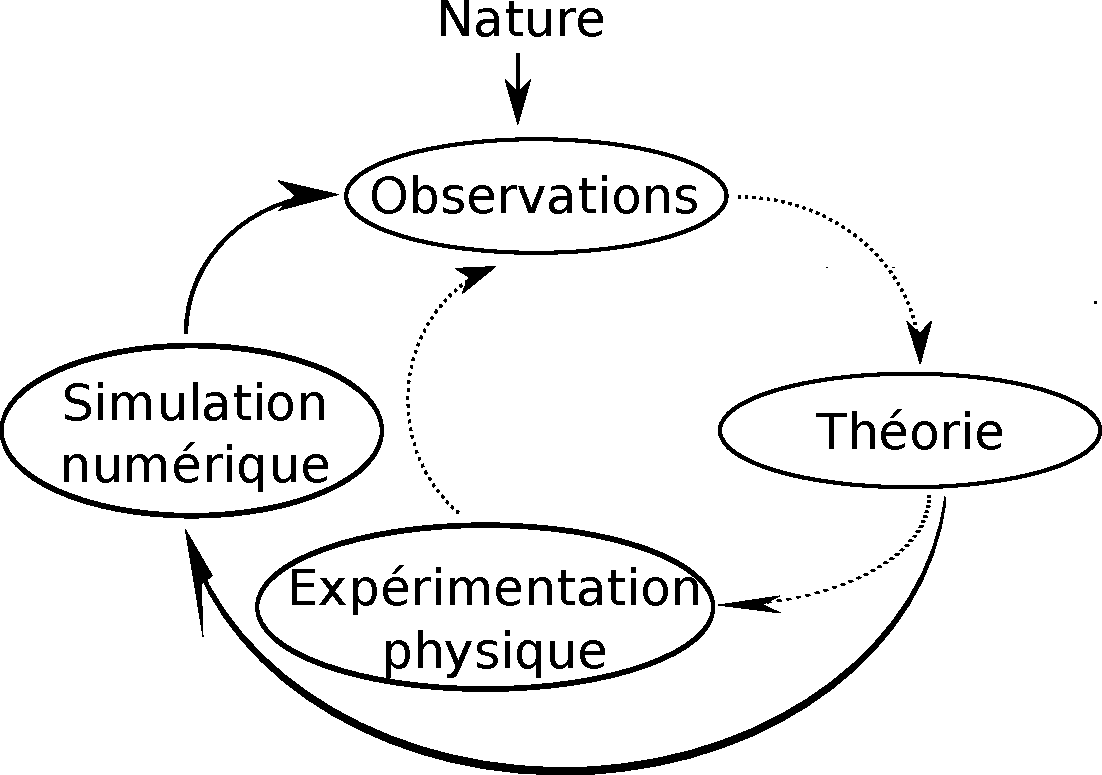
\includegraphics[width=0.9\textwidth]{Science-SimuNum.pdf}
      \end{figure}
      {\tiny (d'après 
        % {\it Parallel Programming in C 
        % with MPI and OpenMP}, 
        M.J. Quinn)} 
    \end{center}
  \end{columns}
\end{exampleblock}

\begin{itemize}
\item[$\leadsto$] 3ème pilier de la science ?
\end{itemize}  
\end{frame}


%%%%%%%%%%%%%%%%%%%%%%%%%%%%%%%%%%%%%%%%%%%%%%%%%%%%%%%%%%%%%%%%%%%%%
\begin{frame}
\frametitle{Les grands domaines d'application du HPC}


\begin{block}{``Grands challenges'' scientifiques}
  \begin{itemize}
  \item Chimie, biologie : dynamique moléculaire 
  \item Bio-informatique : séquençage du génome
  \item Astrophysique : dynamique des  galaxies, de l'Univers  
  \item Climatologie : échanges océan $\leftrightarrow$ atmosphère
  \item Méca. des fluides : écoulements turbulents, combustion
  \item ...
  \end{itemize}
\end{block}

Et aussi : 
\begin{itemize}
\item Géophysique : propagation d'ondes sismiques
\item Industrie automobile : simulation d'accidents 
\item \og \textit{Deep Learning}\fg
\item ... 
\end{itemize}
\end{frame}

%%%%%%%%%%%%%%%%%%%%%%%%%%%%%%%%%%%%%%%%%%%%%%%%%%%%%%%%%%%%%%%%%%%%%

\begin{frame}
\frametitle{Illustration du problème}

\begin{center}
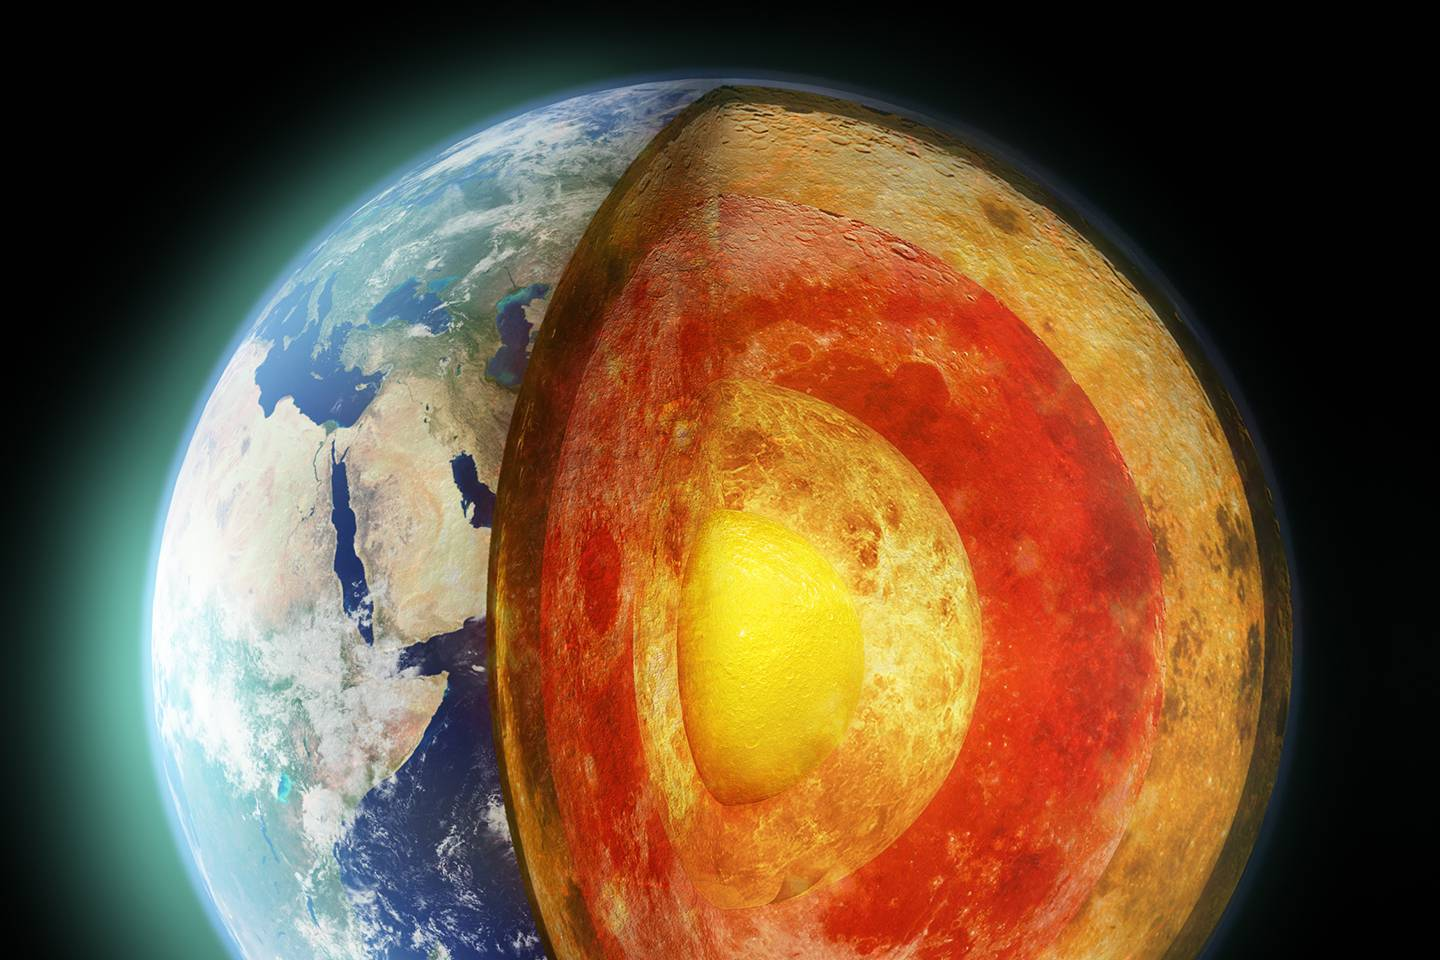
\includegraphics[width=5cm]{earth-core.jpg}
\end{center}

\begin{itemize}
\item surface = 510 millions de km${^2}$, volume $\approx 10^{12}$ km${}^3$
  \medskip
\item Un \texttt{double} par km${}^3$ $\leadsto$ 8 To de mémoire

\item Un \texttt{double} par m${}^2$ $\leadsto$ 4 Po de mémoire
\end{itemize}

\end{frame}

%%%%%%%%%%%%%%%%%%%%%%%%%%%%%%%%%%%%%%%%%%%%%%%%%%%%%%%%%%%%%%%%%%%%%

\begin{frame}
\frametitle{Illustration du problème}

\begin{center}
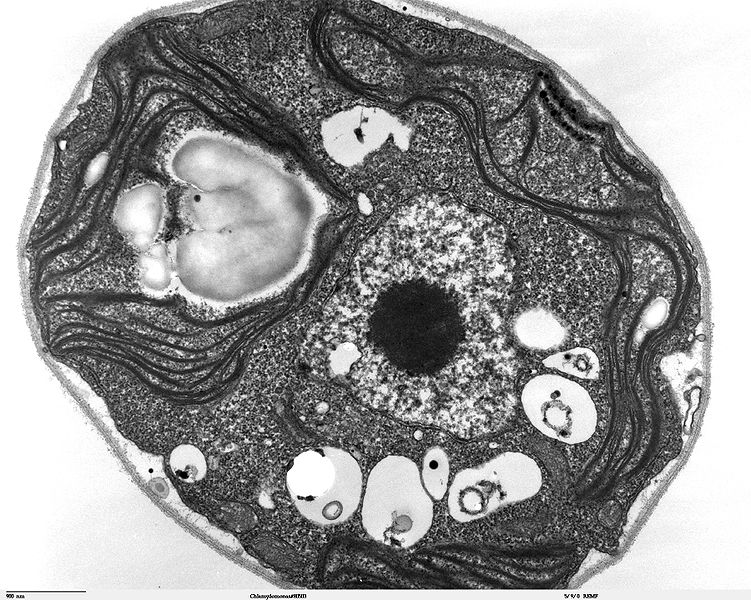
\includegraphics[width=5cm]{cell.jpg}
\end{center}

\begin{itemize}
\item Cellule humaine. Environ $10^{14}$ atomes.
\item 3 $\times$ \texttt{double} $(x, y, z)$ par atome $\leadsto$ 2.4 Po de mémoire
\end{itemize}

\medskip

\begin{alertblock}{Not to mention...}
  \begin{itemize}
  \item $10^{11}$--$10^{12}$ étoiles dans notre galaxie
  \item $10^{11}$--$10^{12}$ galaxies...
  \end{itemize}
\end{alertblock}

\end{frame}


%%%%%%%%%%%%%%%%%%%%%%%%%%%%%%%%%%%%%%%%%%%%%%%%%%%%%%%%%%%%%%%%%%%%%%

\begin{frame}
  \frametitle{Constat \triste}

  \begin{itemize}
  \item Vous savez \textbf{un peu} comment fonctionne un ordinateur
    \begin{itemize}
    \item Mais \red{pas complètement}
    \item Surtout pour les gros
    \end{itemize}

    \medskip
    
  \item Vous n'avez pas été formés à :
    \begin{itemize}
    \item vous \red{préoccuper} des \textbf{performances} de votre code
    \item écrire des programmes \red{efficaces}
    \end{itemize}
    
    \pause
    \bigskip

    \item \Huge \textbf{Time for a change}
    \end{itemize}

\end{frame}

%%%%%%%%%%%%%%%%%%%%%%%%%%%%%%%%%%%%%%%%%%%%%%%%%%%%%%%%%%%%%%%%%%%%%% 

\begin{frame}
  \frametitle{Puissance de calcul}

  \begin{block}{Mesure de performance}
  Unité : FLOP (\textit{Floating Point OPeration}), FLOP/s (ou FLOPS)

  \begin{itemize}
  \item Giga ($10^9 \approx 2^{30}$)
  \item Tera ($10^{12} \approx 2^{40}$)
  \item Peta ($10^{15} \approx 2^{50}$)
  \item Exa  ($10^{18} \approx 2^{60}$) \dots 
  \end{itemize}
\end{block}

\bigskip

\begin{itemize}
\item Machines pour gros calculs = \textbf{machines \red{parallèles}}

  \medskip

  \item Le parallélisme est une \textbf{tendance de fond}
  \end{itemize}
\end{frame}


%%%%%%%%%%%%%%%%%%%%%%%%%%%%%%%%%%%%%%%%%%%%%%%%%%%%%%%%%%%%%%%%%%%%%%
\section{Matériel pour le HPC}

%%%%%%%%%%%%%%%%%%%%%%%%%%%%%%%%%%%%%%%%%%%%%%%%%%%%%

\begin{frame}
  \frametitle{PC des années 1990}
  \framesubtitle{Le seul que vous savez vraiment programmer}
  
  \centering
  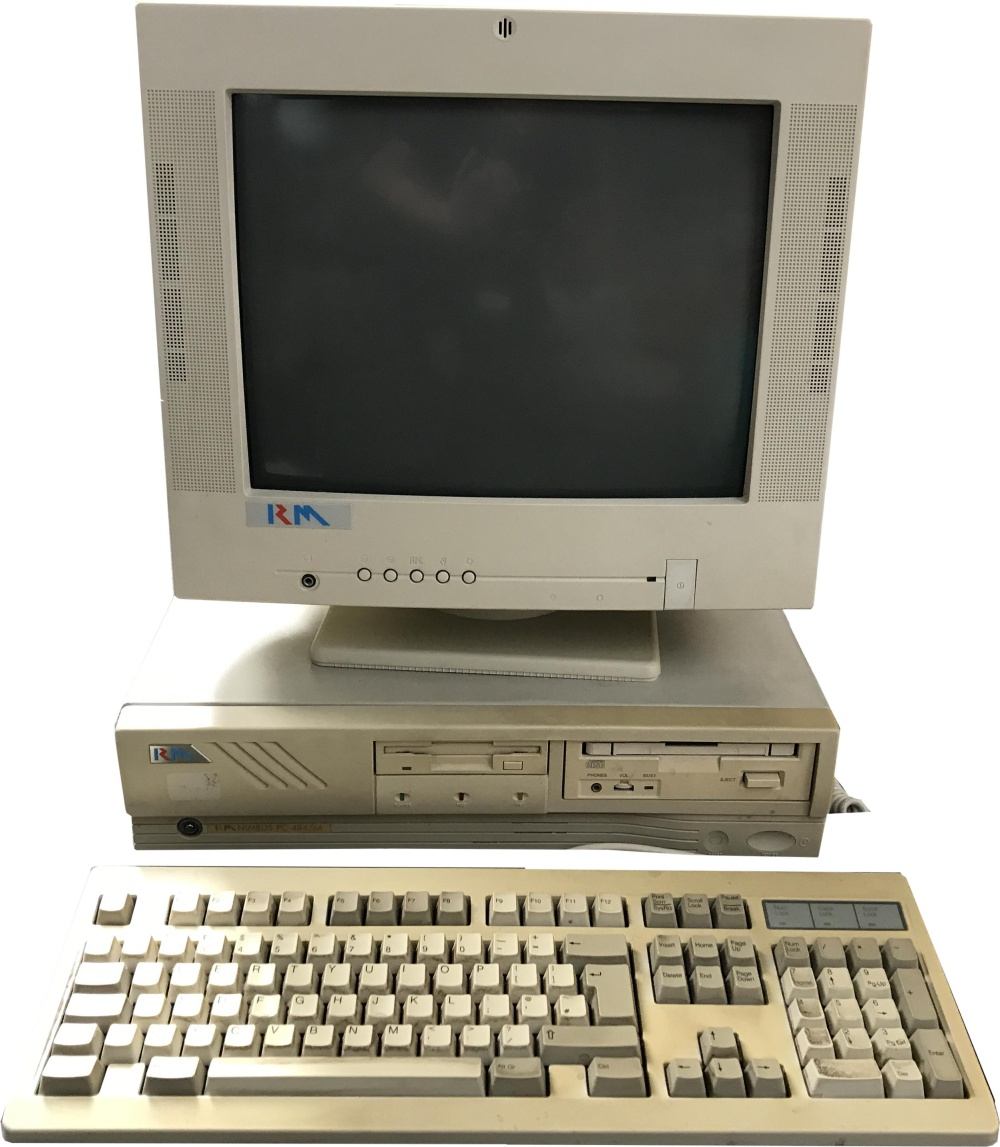
\includegraphics[height=0.5\textheight]{old_pc}
  \hfill
  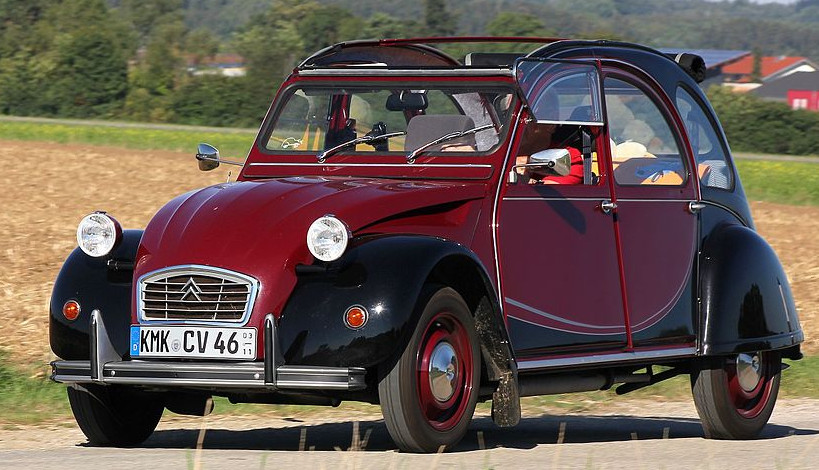
\includegraphics[width=6cm]{2cv}

  \bigskip

  1 coeur, 25Mhz, 16Ko de Cache, 4Mo de RAM
\end{frame}

%%%%%%%%%%%%%%%%%%%%%%%%%%%%%%%%%%%%%%%%%%%%%%%%%%%%%%

\begin{frame}
  \frametitle{Laptop moderne}
  \framesubtitle{Celui que vous avez, avec un peu de chance}
  
  \centering
  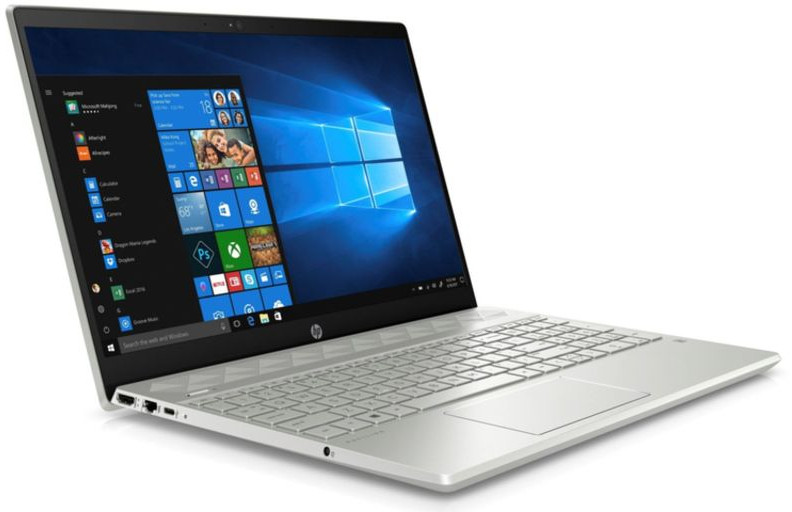
\includegraphics[width=5cm]{laptop}%
  %\hfill%
  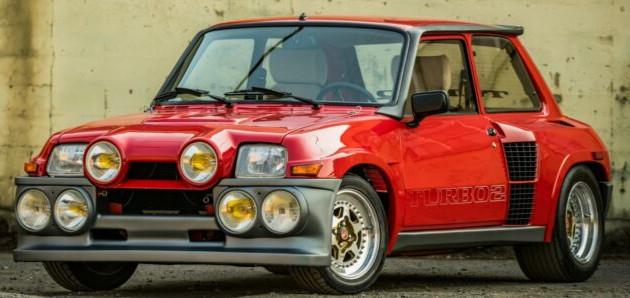
\includegraphics[width=6cm]{r5maxi}

    \bigskip

  4 coeurs, 4Ghz, 8Mo de cache, 16Go de RAM (2 canaux)
\end{frame}


\begin{frame}
  \frametitle{PC de gamer}
  \framesubtitle{Pour ceux qui se croient malin en faisant de l'IA}
  
  \centering
  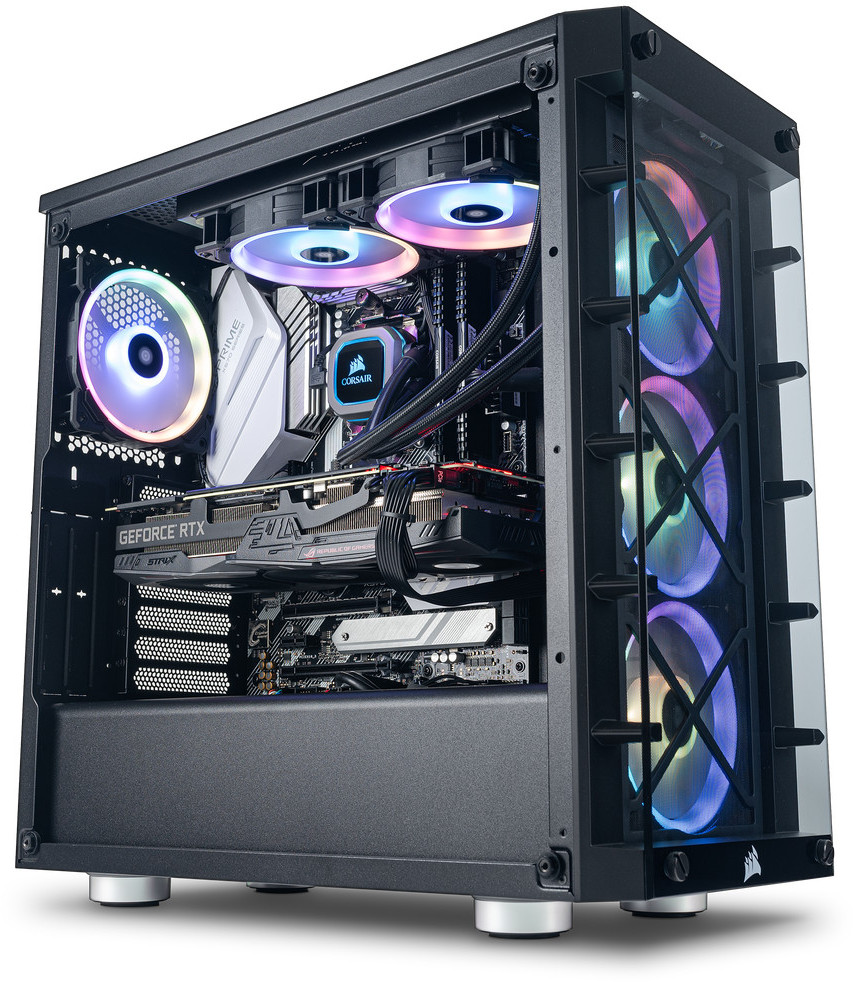
\includegraphics[width=5cm]{gamer}%
  \hfill%
  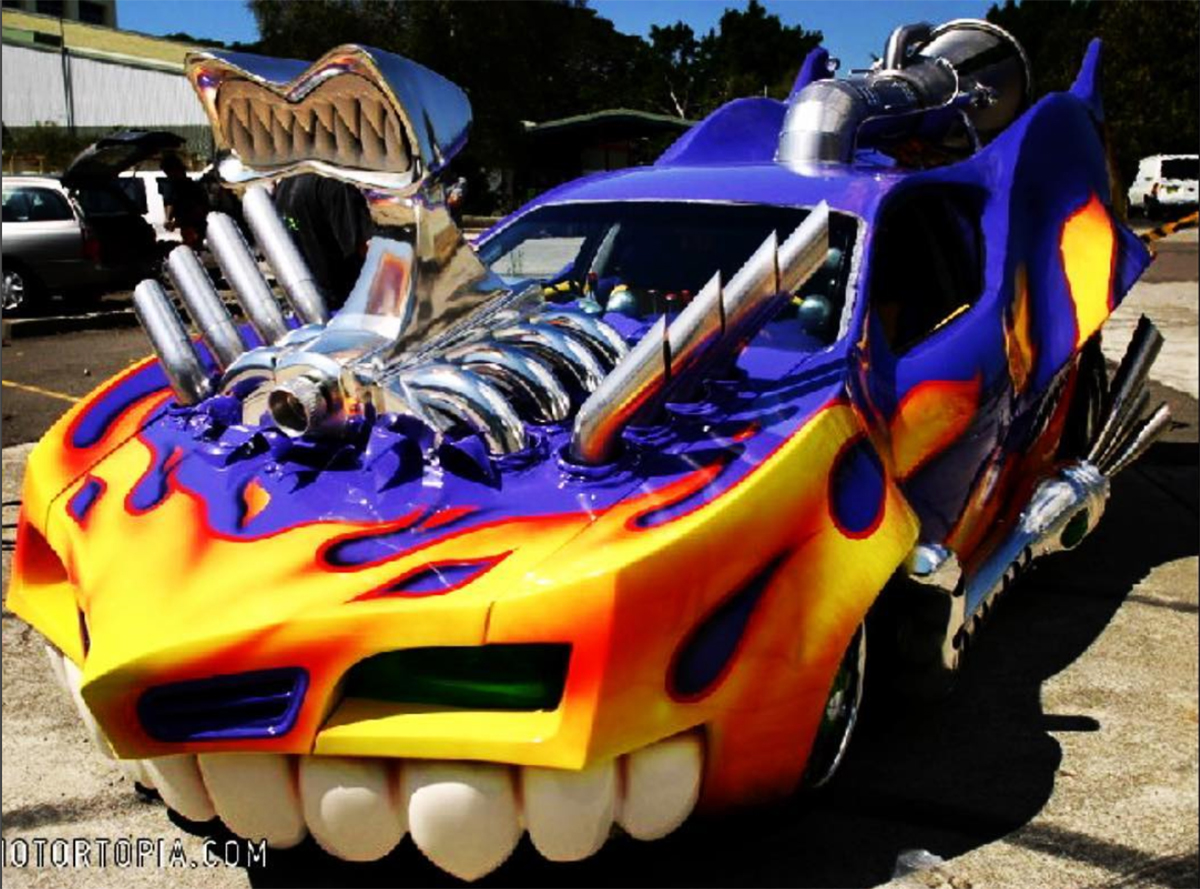
\includegraphics[width=5.5cm]{tuning}

    \bigskip

    10--16 coeurs, 4Ghz, 16Mo de cache, 32Go de RAM (2 canaux)
\end{frame}


\begin{frame}
  \frametitle{Serveur de calcul}
  \framesubtitle{Now we're talking}
  
  \centering
  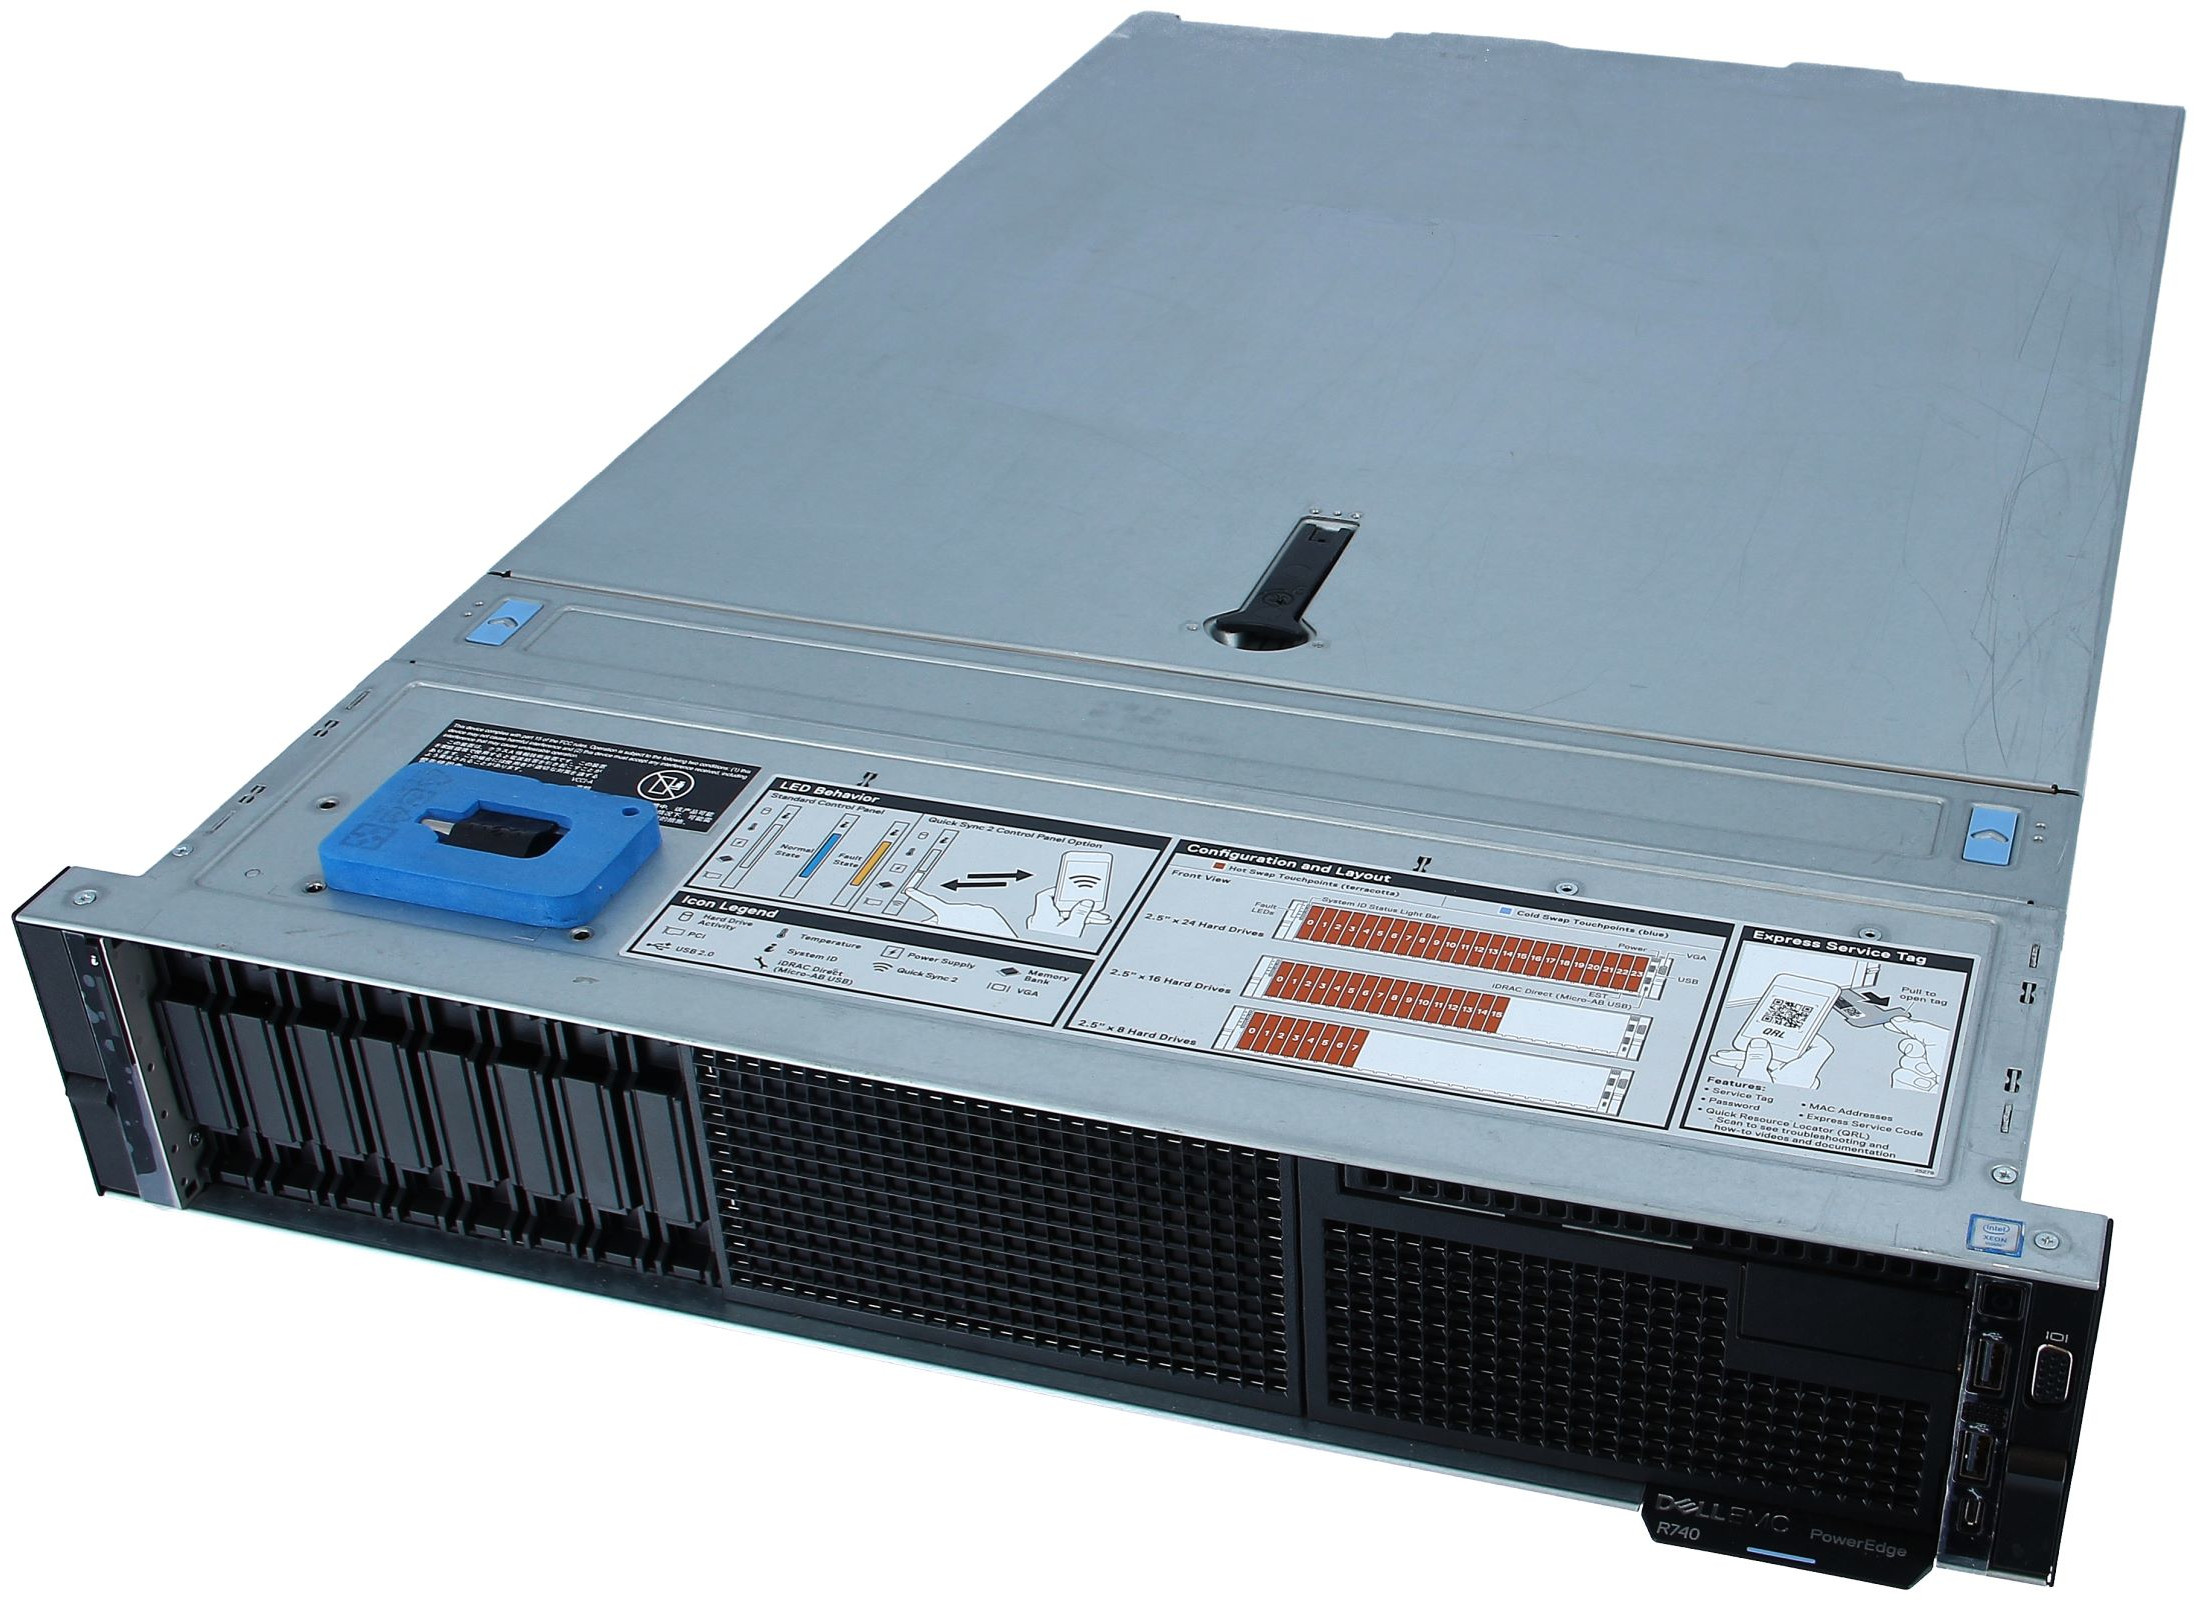
\includegraphics[width=5cm]{dell1}
  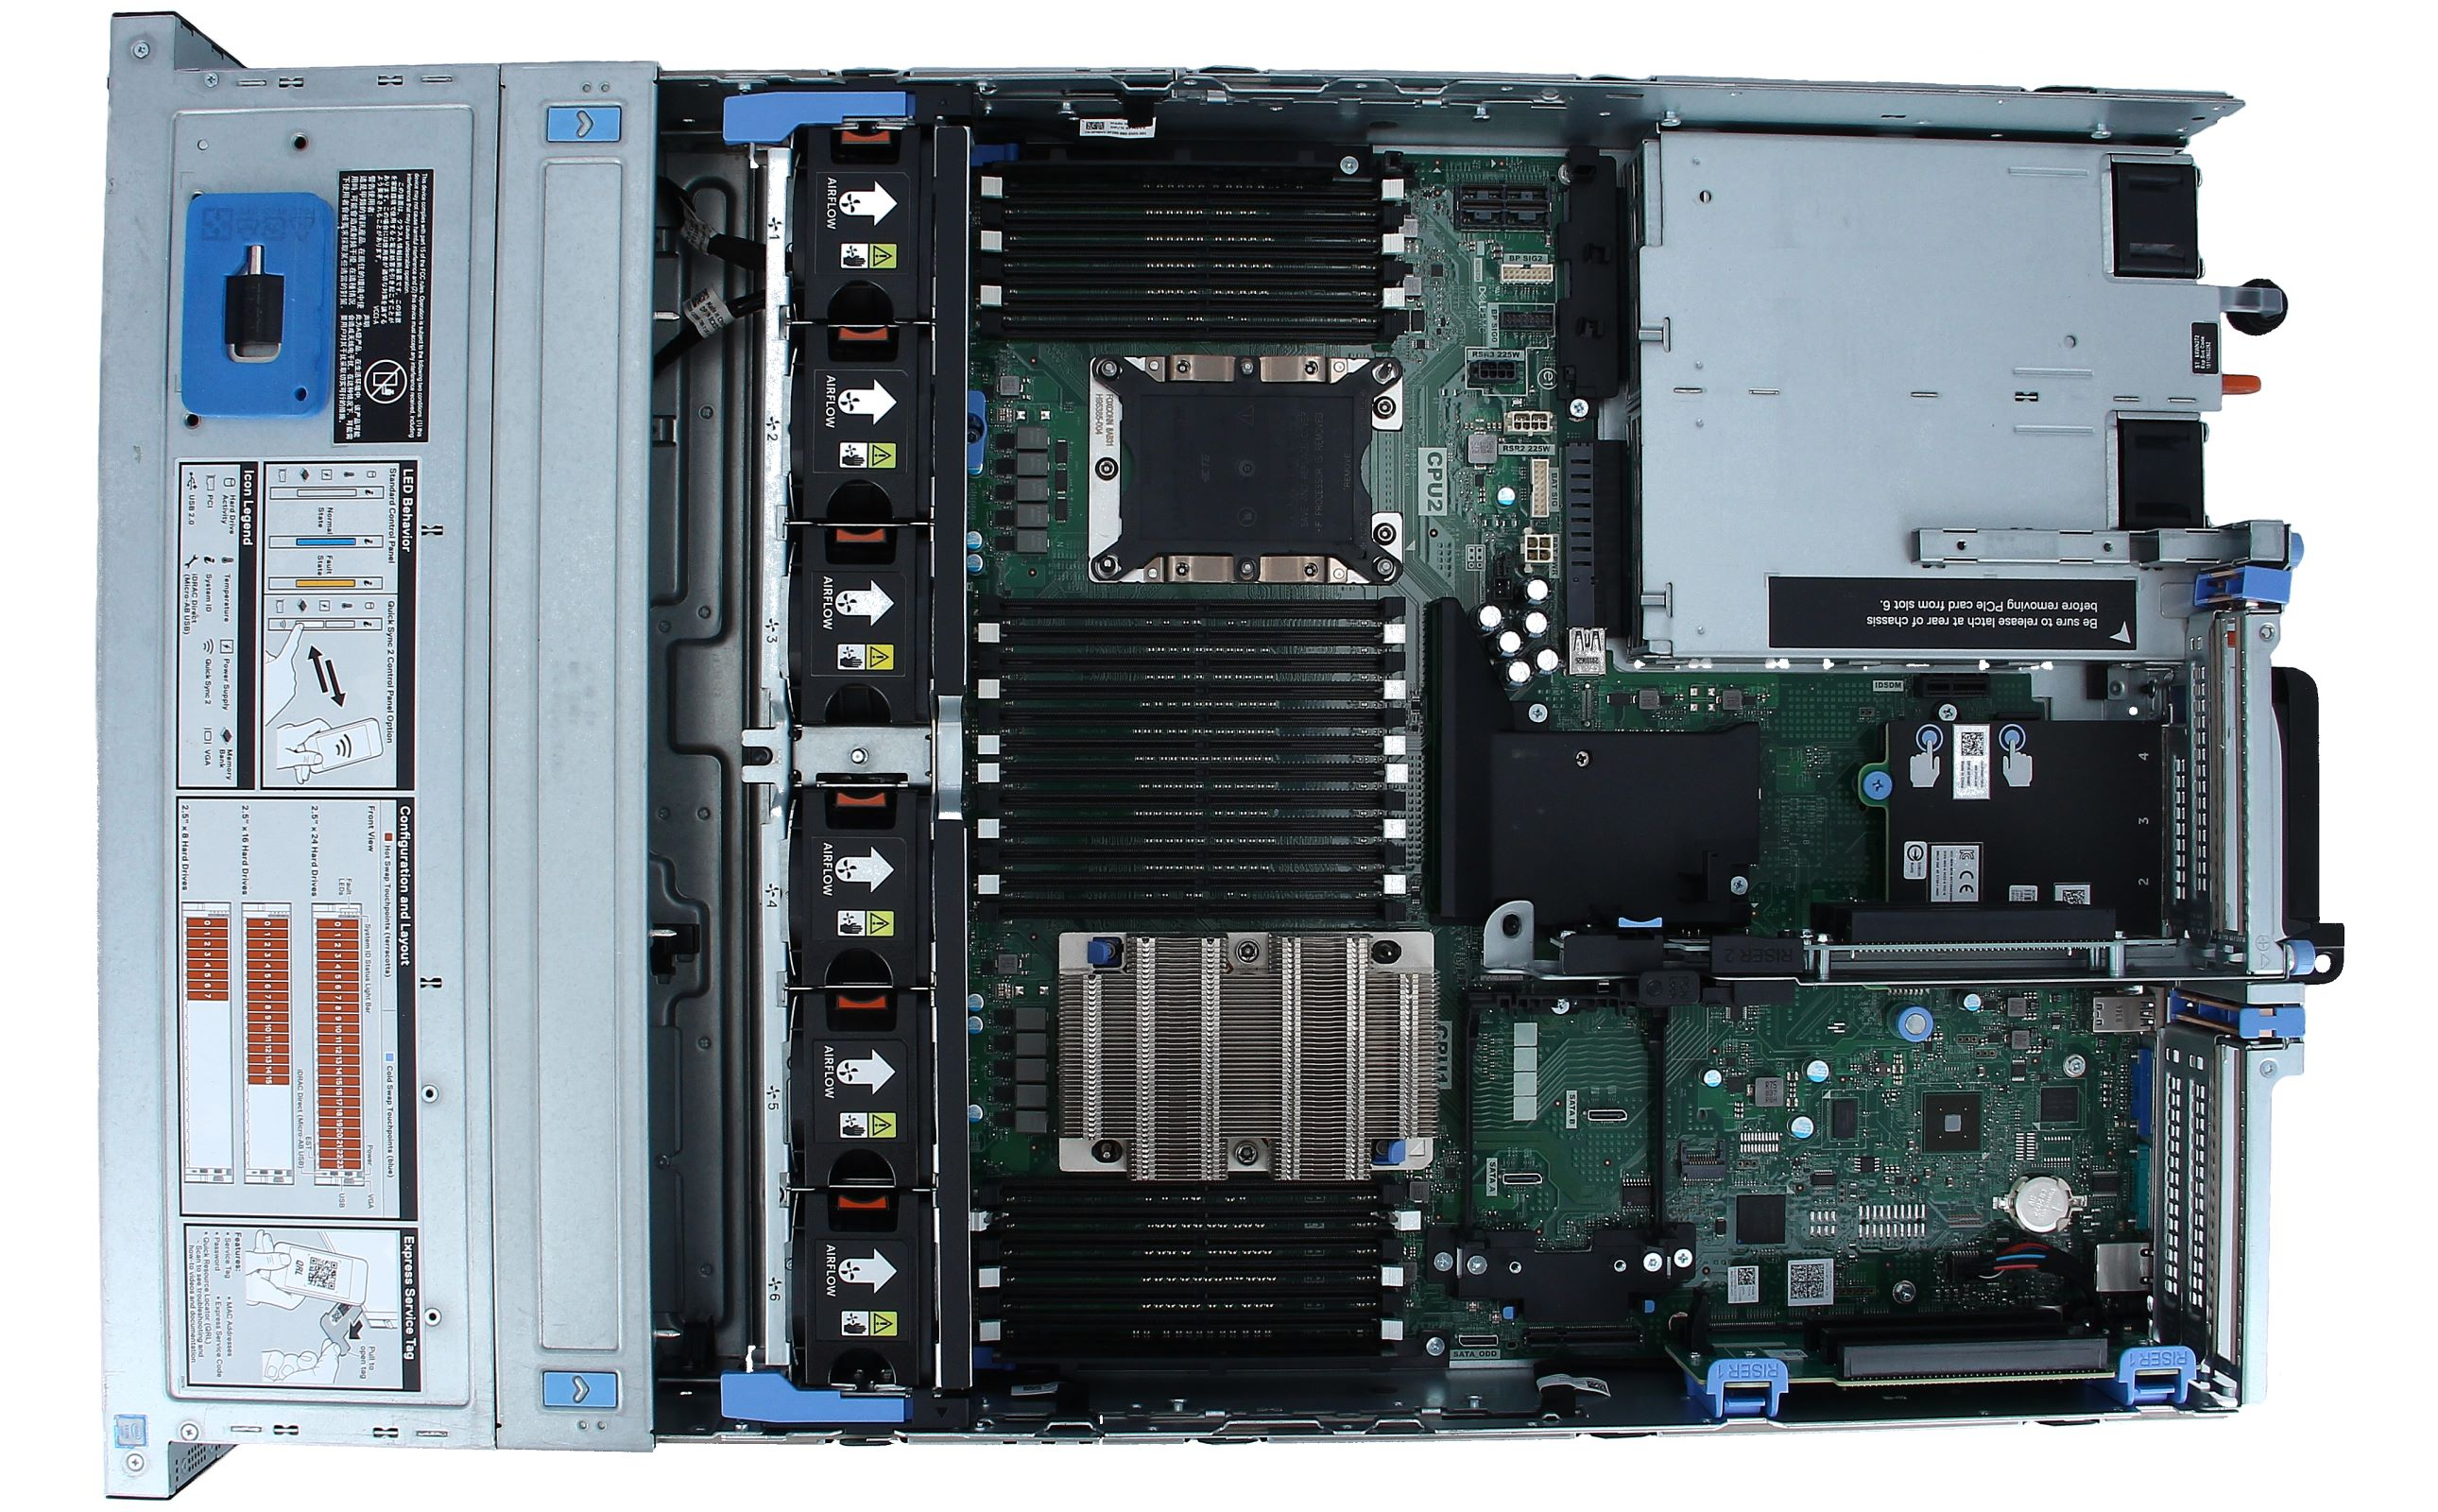
\includegraphics[width=5cm]{dell2}


  
  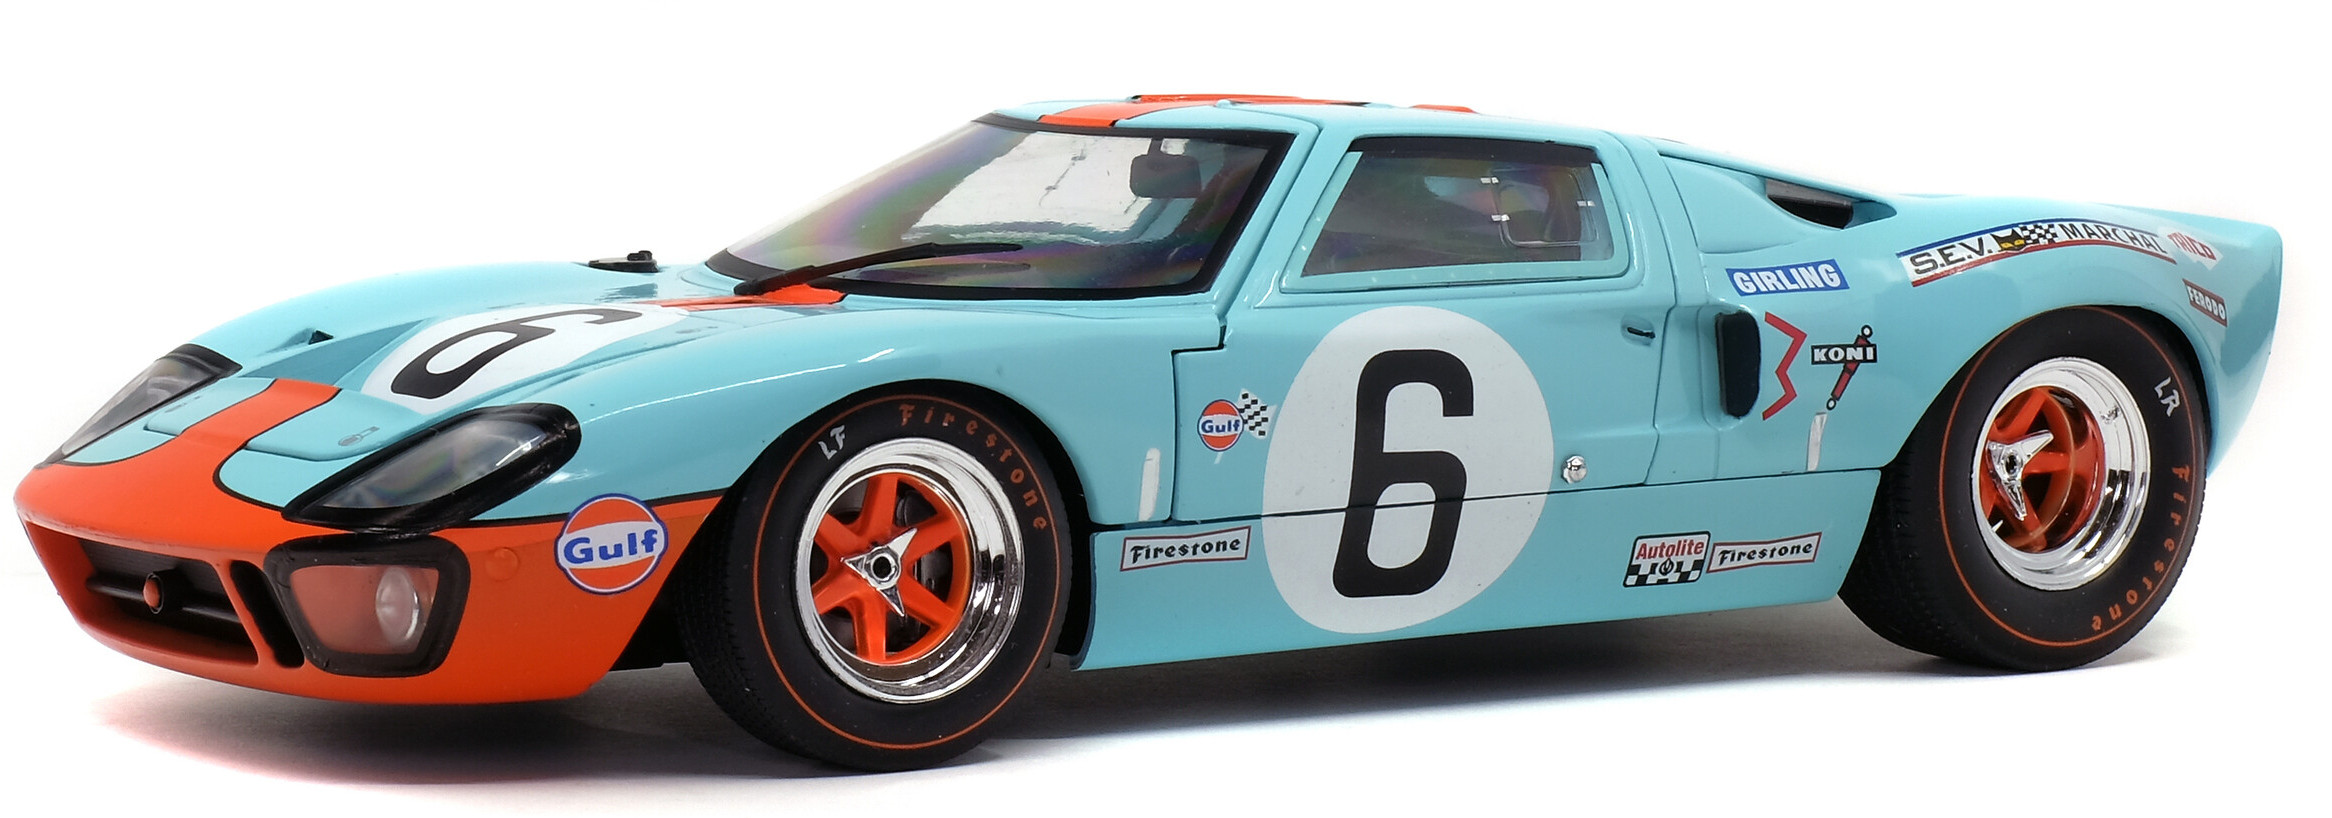
\includegraphics[width=8cm]{gt40}

  \bigskip

  2 CPUs, 32--128 coeurs, 2.5Ghz, 192Go RAM ($2\times 6$ canaux)
\end{frame}


\begin{frame}
  \frametitle{Machine de HPC}
  \framesubtitle{Rare et cher}
  
  \centering
  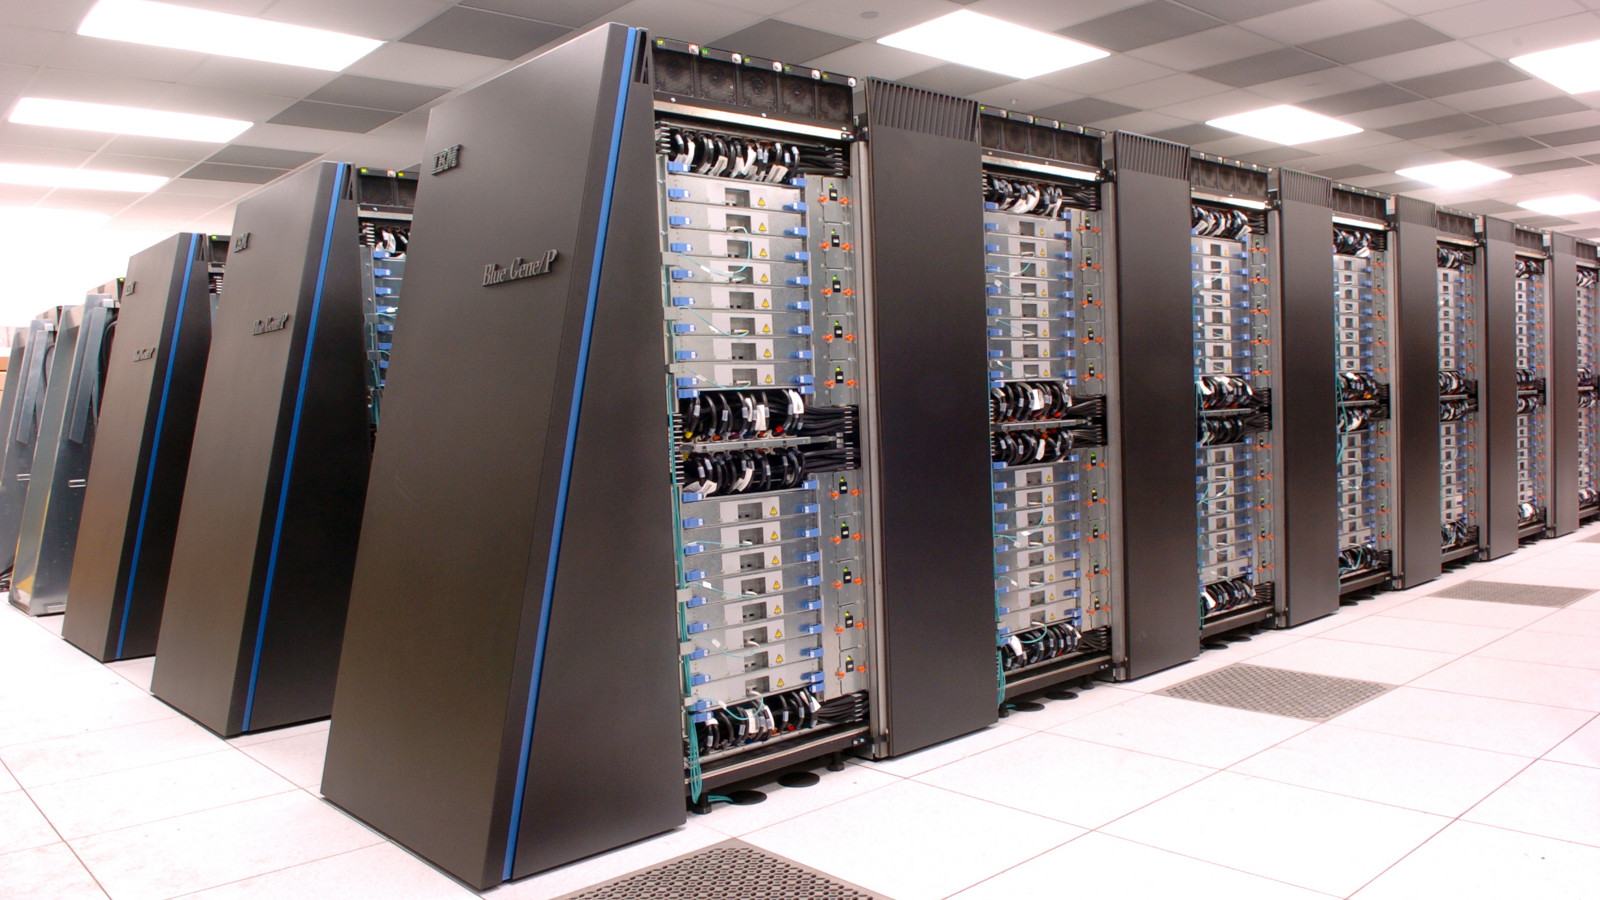
\includegraphics[width=7cm]{bgp}
  \hfill
  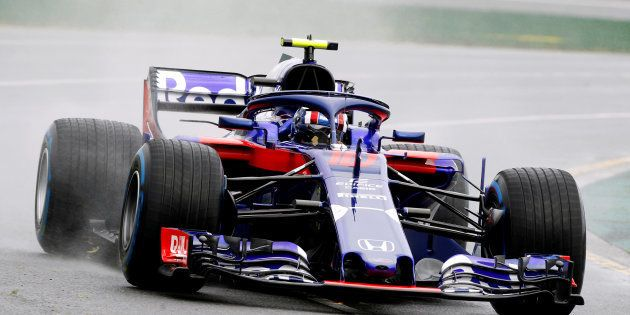
\includegraphics[width=7cm]{f1}

  \bigskip
  
  1000--10000000 coeurs. coût variable de $10^{6}$ à $10^{9}$ euros
\end{frame}

%%%%%%%%%%%%%%%%%%%%%%%%%%%%%%%%%%%%%%%%%%%

%%%%%%%%%%%%%%%%%%%%%%%%%%%%%%%

\begin{frame}
  \frametitle{Une machine de HPC : \texttt{Turing}}
  \framesubtitle{IBM BlueGene/Q (2012--2019) @ IDRIS (CNRS)}
  
  \begin{center}
    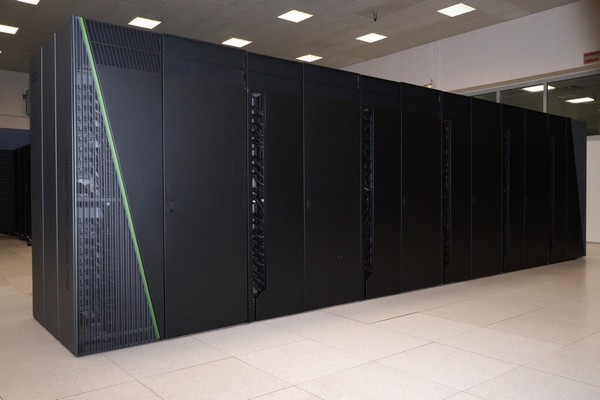
\includegraphics[height=6.5cm]{turing}
  \end{center}
\end{frame}


\begin{frame}
  \frametitle{Une machine de HPC : \texttt{Turing}}
  \framesubtitle{IBM BlueGene/Q (2012--2019) @ IDRIS (CNRS)}

  6 baies, 98~304 coeurs (``petit'') $\leadsto$ \texttt{Sequoia} (USA) en a 1~572~864
  
  \begin{center}
    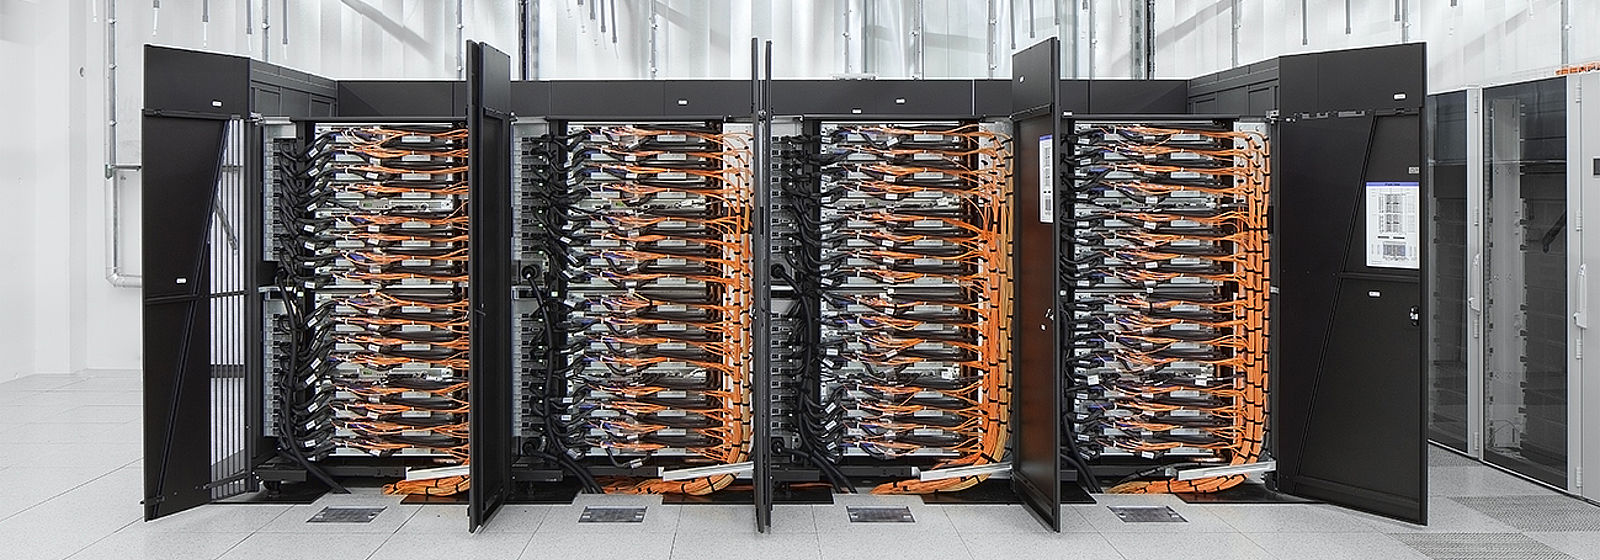
\includegraphics[width=\textwidth]{bgq}
  \end{center}
\end{frame}

\begin{frame}
  \frametitle{Une machine de HPC : \texttt{Turing}}
  \framesubtitle{IBM BlueGene/Q (2012--2019) @ IDRIS (CNRS)}
  
  \begin{columns}
    \begin{column}{0.33\textwidth}
      1 baie =
      \begin{itemize}
      \item 16 \textit{node cards}
      \item + alimentation
      \item + \textit{water cooling}
      \item + noeuds I/O
      \end{itemize}

      \bigskip
      
      Total =
      \begin{itemize}
      \item 1024 noeuds
      \item 16 384 coeurs
      \item 16 To de RAM
      \end{itemize}
      
    \end{column}
      
    \begin{column}{0.66\textwidth}
      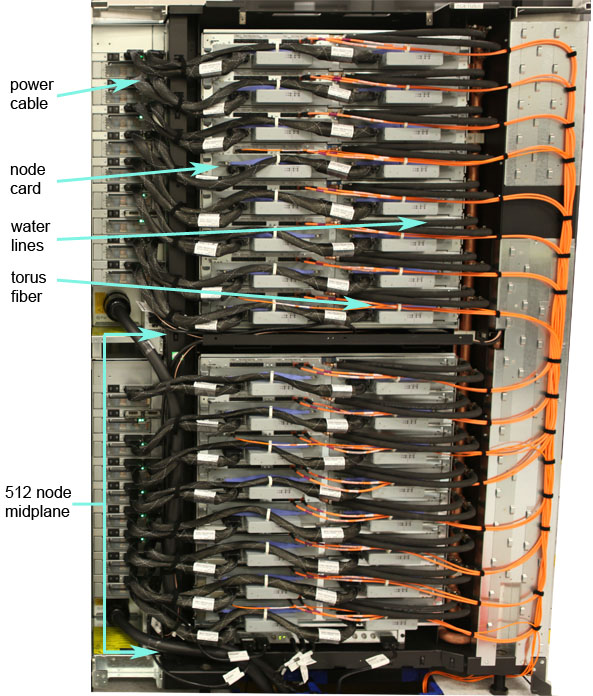
\includegraphics[height=7.5cm]{bgqMidplane}
    \end{column}
  \end{columns}
\end{frame}


\begin{frame}
  \frametitle{Une machine de HPC : \texttt{Turing}}
  \framesubtitle{IBM BlueGene/Q (2012--2019) @ IDRIS (CNRS)}
  
  1 \textit{node card} = 32 \textit{compute cards}
  
  \begin{center}
    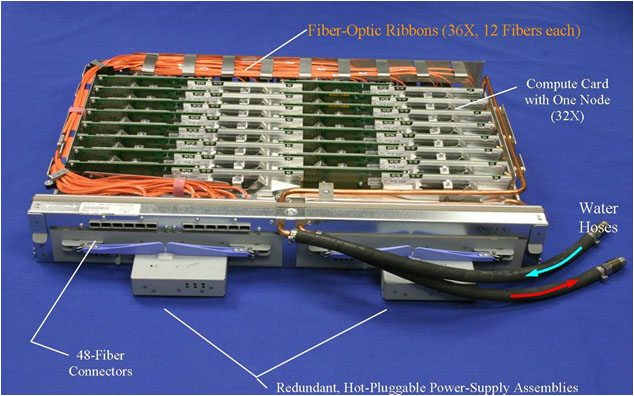
\includegraphics[height=6.5cm]{bgqNodeCard}
  \end{center}
\end{frame}


\begin{frame}
  \frametitle{Une machine de HPC : \texttt{Turing}}
  \framesubtitle{IBM BlueGene/Q (2012--2019) @ IDRIS (CNRS)}
  
  1 \textit{compute card} =
  \begin{itemize}
  \item 1 processeur (PowerPC A2, 1.6Ghz, 16 coeurs)
  \item 16Go de RAM ECC (36 chips de 512Mo)
  \end{itemize}

  \begin{center}
    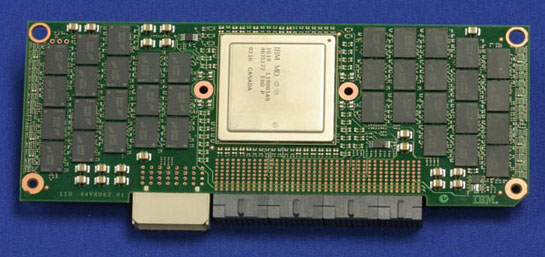
\includegraphics[width=\textwidth]{bgqComputeCard}
  \end{center}
\end{frame}

\begin{frame}
  \frametitle{Une machine de HPC : \texttt{Turing}}
  \framesubtitle{IBM BlueGene/Q (2012--2019) @ IDRIS (CNRS)}

    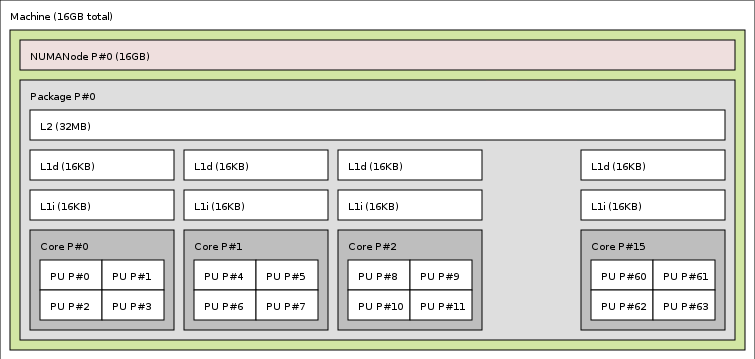
\includegraphics[width=\textwidth]{lstopo_bgq}
\end{frame}

%%%%%%%%%%%%%%%%%%%%%%%%%%%%%%%%%%%%%%%%%%%%%%%%%%%%%

\begin{frame}
  \frametitle{Pas des ordinateurs \og normaux \fg}

  \begin{center}
    \begin{tikzpicture}
      \node at (6cm, 0) {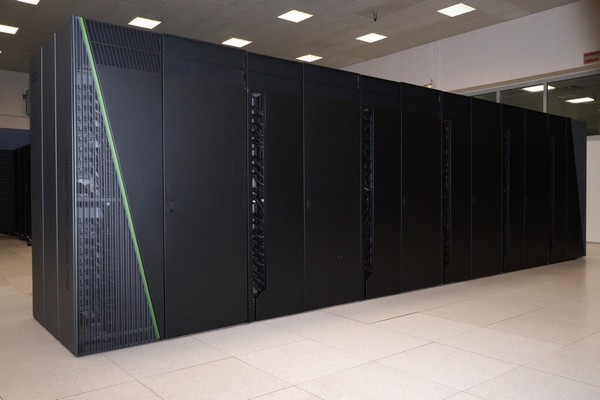
\includegraphics[width=4cm]{turing}};
      \node at (0, 0) {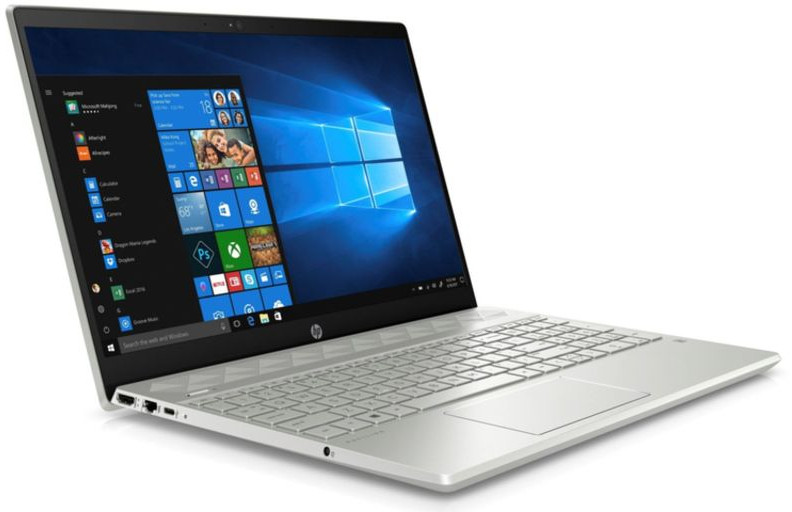
\includegraphics[width=3cm]{laptop}};

      \node at (0cm, -4cm) {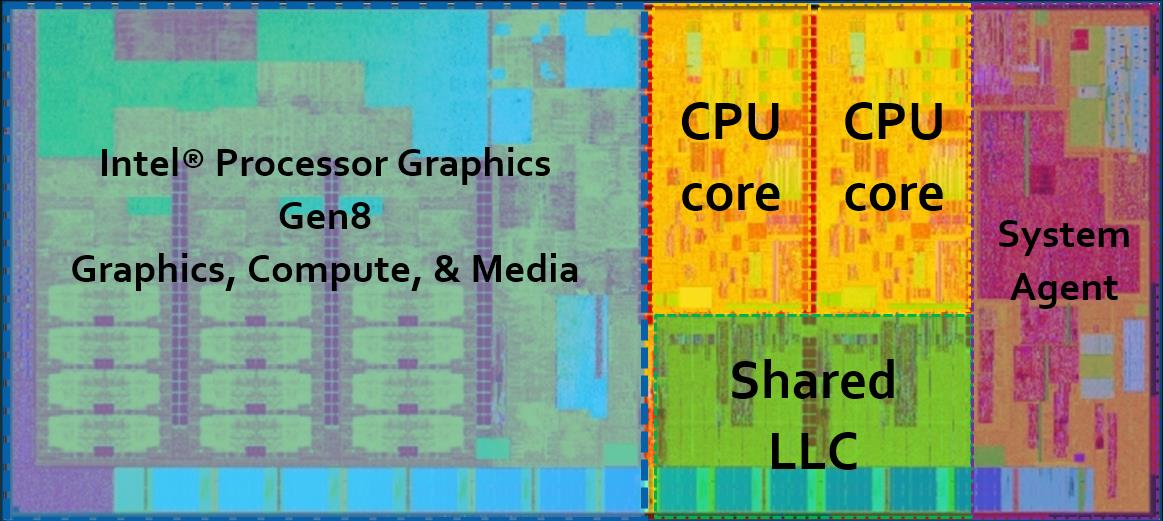
\includegraphics[width=4cm]{i5-silicon-die-layout.jpg}};
      \node at (6cm, -4cm) {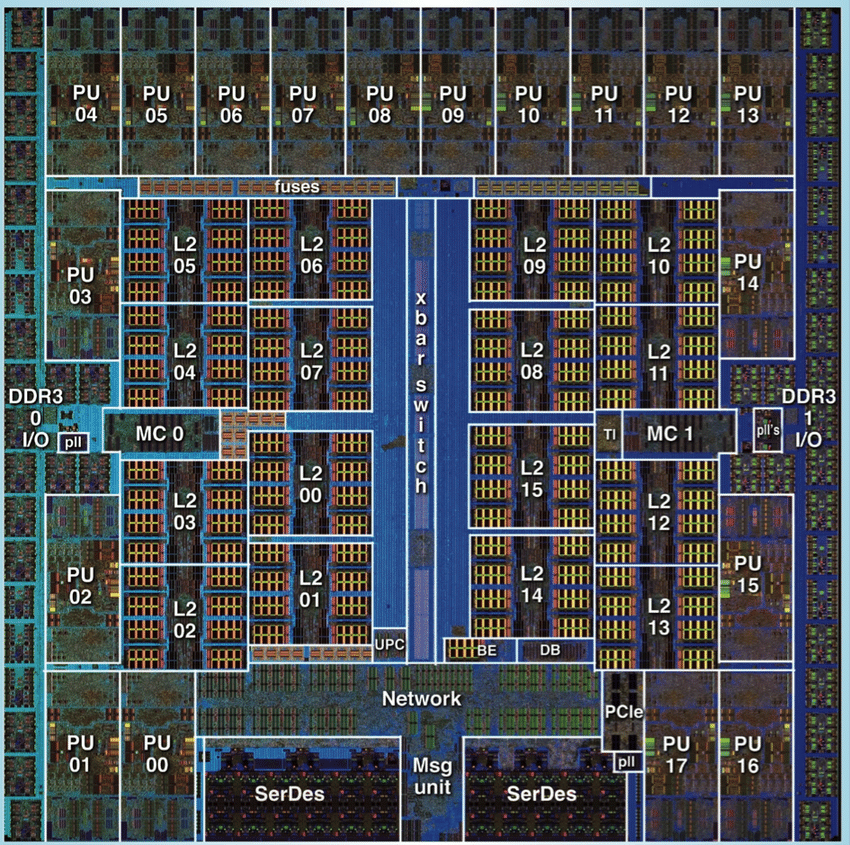
\includegraphics[width=5cm]{die-bgq.png}};
    \end{tikzpicture}
  \end{center}
\end{frame}

%%%%%%%%%%%%%%%%%%%%%%%%%%%%%%%%%%%%%%%%%%%%%%%%%%%%%

\begin{frame}
  \frametitle{Quelques exemples (au CNRS)}

  \begin{enumerate}
  \item \texttt{Turing} (IDRIS / CNRS, 2012--2019), 1.2 PetaFLOPS
    \begin{itemize}
    \item IBM BlueGene/Q ($\approx$ 20 millions \euro)
    \item 6144 noeuds, 98 304 coeurs, 98To de RAM
      \begin{itemize}
      \item 16Go + 1 $\times$ IBM PowerPC A2, 16 coeurs @ 1.6 Ghz
      \item 1 CPU = ??? \euro = 200 GigaFLOPS
      \end{itemize}
    \item Réseau = ``maison'', tore 5D, 10 $\times$ 2Go/s par noeud.
    \item 600kW (cold water cooling)
    \end{itemize}

    \medskip\pause

  \item<2-> \texttt{Jean-Zay} (IDRIS / CNRS, 2019--), 28 PetaFLOPS
    \begin{itemize}
    \item HPE SGI 8600 (25 millions \euro)
    \item 1528 noeuds ``CPU'' $\rightarrow$ 61~120 coeurs, 4.9 PetaFLOPS
      \begin{itemize}
        \item 192Go + 2 $\times$ Intel Xeon Gold 6248, 20 coeurs, 2.5Ghz
        \item 1CPU = 3000\euro = 1.6 TeraFLOPS
        \end{itemize}
    \item<3-> 662 noeuds ``GPU'' $\rightarrow$ 199~040 coeurs, 21.5 PetaFLOPS
      \begin{itemize}
      \item idem + 4 $\times$ NVIDIA V100 SMX2 16/32Go, 80 coeurs
      \item 1 GPU = 8500\euro = 8 TeraFLOPS
      \end{itemize}
    \item réseau = Intel OmniPath 100Gbit/s
    \item $\approx$ 1MW (warm water cooling)
    \end{itemize}
  \end{enumerate}
\end{frame}

%%%%%%%%%%%%%%%%%%%%%%%%%%%%%%%%%%%%%%%%%%%%%%

\begin{frame}
  \frametitle{Quelques exemples (TOP 500)}

  \begin{enumerate}
  \item \#2 = \texttt{Summit} (DoE, USA, 2018--), 200 PetaFLOPS
    \begin{itemize}
    \item IBM  ($\approx$ \$ 500 millions)
    \item 4~608 noeuds
      \begin{itemize}
      \item $2 \times$ IBM Power9, 22 coeurs, 3Ghz
      \item $6 \times$ NVIDIA V100 16Go
      \item 512Go DDR4 + 96Go HBM + 1.6To non-volatile memory
      \item 1 noeud $\approx$ 120~000\euro = 42 TeraFLOPS
      \end{itemize}
    \item[$\rightarrow$] 2.8Po de RAM, 202~752 coeurs CPU, 2~211~840 coeurs GPU
    \item Réseau = Infiniband 100Gb/s
    \item 13MW 
    \end{itemize}

    \medskip\pause

  \item \#6 = \texttt{Frontera} (Univ. Texas, 2019--), 38.7 PetaFLOPS
    \begin{itemize}
    \item Dell ($\approx$ \$60 millions)
    \item 8008 noeuds
      \begin{itemize}
        \item 192Go + 2 $\times$ Intel Xeon Platinum 8280, 28 coeurs, 2.7Ghz
        \item 1 CPU = 10~000\euro = 2.4 TeraFLOPS
        \end{itemize}
      \item[$\rightarrow$] 1.5Po RAM, 448~448 coeurs
    \item réseau = Infiniband 100Gbit/s
    \end{itemize}
  \end{enumerate}
\end{frame}

%%%%%%%%%%%%%%%%%%%%%%%%%%%%%%%%%%%%%%%%%%%%%%%%%%%

\begin{frame}
  \frametitle{Et bien sûr...}

  \begin{itemize}
  \item \#1 = \texttt{Fugaku} (RIKEN, Japon, 2021--), 550 PetaFLOPS
    \begin{itemize}
    \item Fujitsu ($\approx$ 900 millions \euro)
    \item $\geq$ 150~000 noeuds
      \begin{itemize}
      \item 32Go HBM2 + $1 \times$ Fujitsu A64FX (arm), 48 coeurs, 2Ghz
      \item 1 CPU = 2.7 TeraFLOPS
      \end{itemize}
    \item[$\rightarrow$] 4.8Po de RAM, 7~200~000 coeurs
    \item Réseau = Tore 6D (tofu)
    \end{itemize}
  \end{itemize}

  \bigskip

  Bientôt des machines (pre-)exascale en Europe
\end{frame}

%%%%%%%%%%%%%%%%%%%%%%%%%%%%%%%%%%%%%%%%%%%%%%%%%%%%%

\begin{frame}
  \frametitle{Votre futur (proche)...}

  \begin{center}
    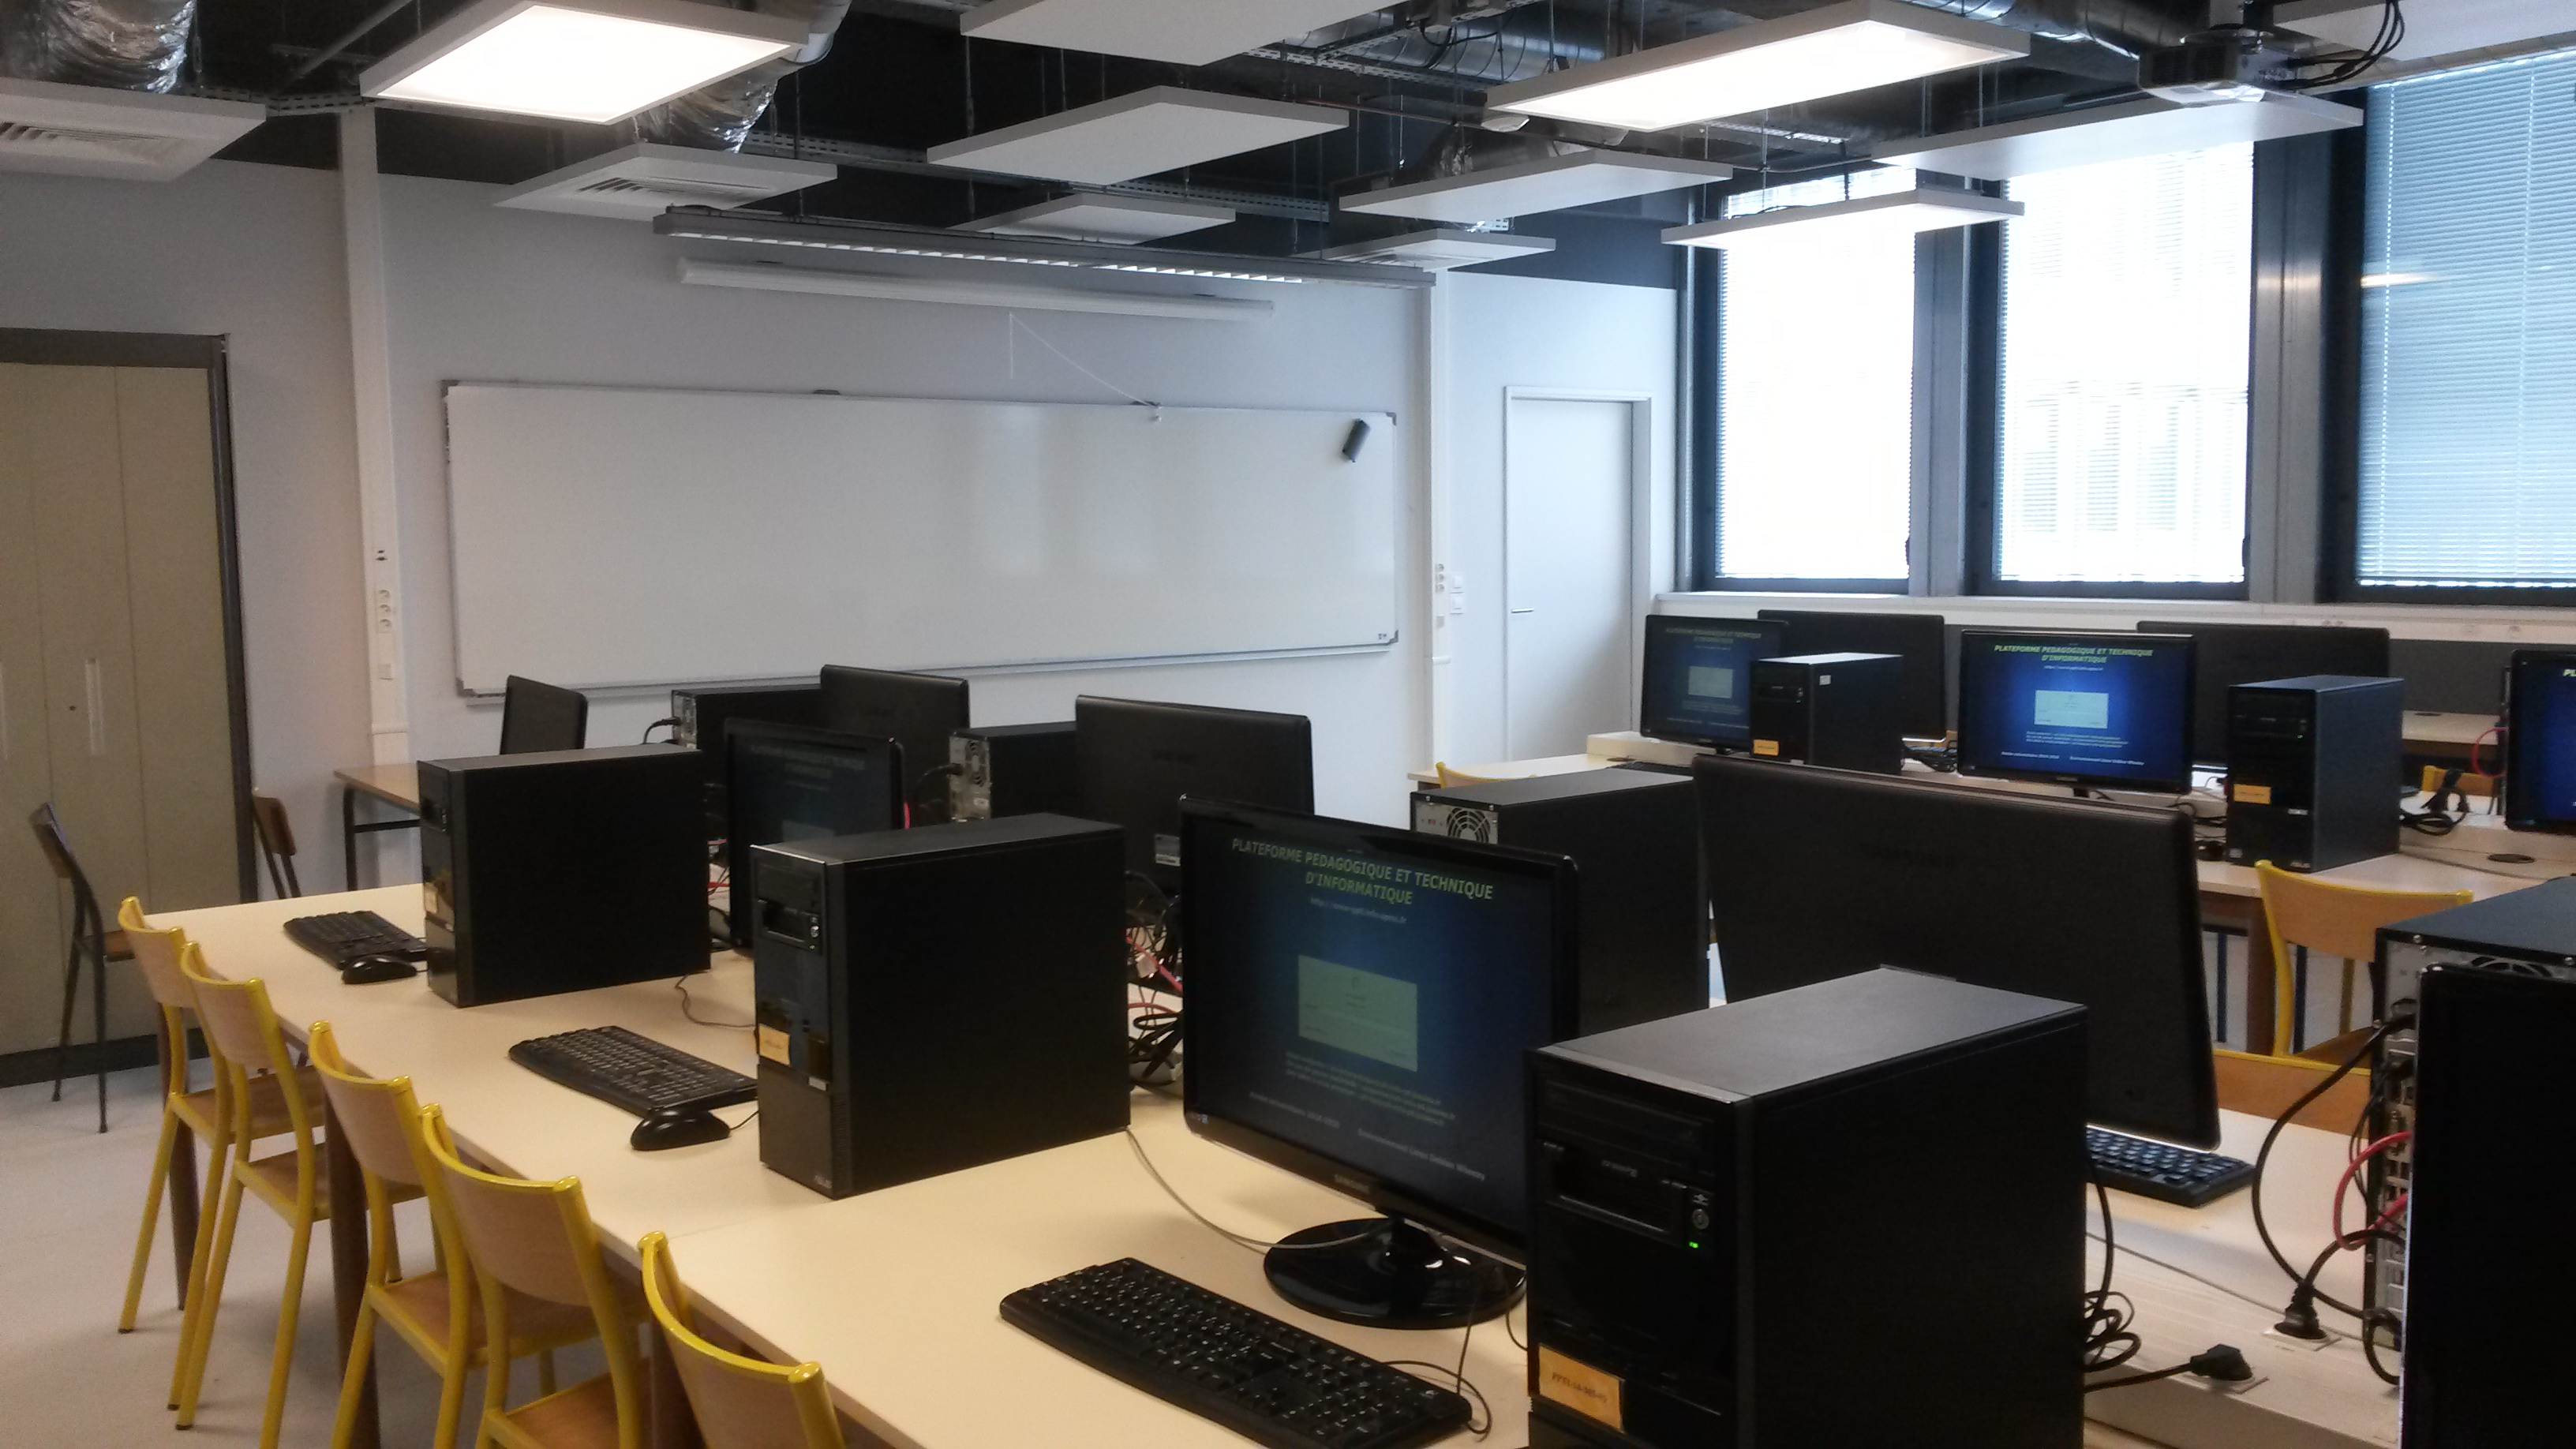
\includegraphics[height=4cm]{ppti}
  \end{center}
  
  \begin{itemize}
  \item \#9999 = Une salle de TP, $\approx 0.8$ TeraFLOPS
    \begin{itemize}
    \item 16 noeuds
      \begin{itemize}
      \item 4Go RAM + $1 \times$ Core i5 (4 coeurs)
      \item 1 CPU = 50 GigaFLOPS
      \end{itemize}
    \item[$\rightarrow$] 64Go de RAM, 64 coeurs
    \item Réseau = (gigabit ?) ethernet
    \end{itemize}
  \end{itemize}

\end{frame}

%%%%%%%%%%%%%%%%%%%%%%%%%%%%%%%%%%%%%%%%%%%%%%%%%%%%% 

\begin{frame}
  \frametitle{Grande variété architecturale}

  \begin{block}{Comment obtenir de la puissance de calcul ?}
    \begin{itemize}
    \item CPUs les plus puissants possible (\texttt{frontera})
    \item Plein de CPUs peu puissants (IBM BlueGene)
    \item Accélérateurs matériels (GPU) (\texttt{summit}, \texttt{jean-zay})
    \item Convergence CPU/GPU (\texttt{fugaku})
    \end{itemize}
  \end{block}

  \bigskip

  \begin{alertblock}{Difficulté de portage}
    À l'extrême, des programmes sont parfois optimisés pour UNE machine donnée.
  \end{alertblock}  
\end{frame}



%%%%%%%%%%%%%%%%%%%%%%%%%%%%%%%%%%%%%%%%%%

\begin{frame}
  \frametitle{Histoire du Top500}

  \small
  \begin{tabular}{|l||c|r|r|r|r|r|}
  \hline
  Machine             & Année & nodes   & $M$/node & FLOPS \\
  \hline\hline
Fugaku                & 2020 & 158 976	& 32G	   &   430P  \\
Summit                & 2018 &   4 608	& 608G	   &   150P  \\
Sunway TaihuLight     & 2016 &  40 960	& 32G	   &    93P  \\
Tiahne-2A             & 2013 &  16 000	& 88G	   &    62P  \\
Titan                 & 2012 &  18 688	& 38G	   &    18P  \\
Sequoia	              & 2012 &  98 304	& 16G	   &    17P  \\
K computer            & 2011 &  82 944	& 16G	   &    11P  \\
Tiahne-1A             & 2010 &   7 168	& 32G	   & 2 566T  \\
Jaguar                & 2009 &  18 688	& 16G	   & 1 941T  \\
Roadrunner            & 2008 &   3 240	& 32G	   & 1 105T  \\
BlueGene/L            & 2004 & 106 496	& 512M	   &   478T  \\
Earth Simulator       &	2002 &     640	& 16G	   &    39T  \\
ASCI White            &	2000 &     512	& 16G	   &  7226T  \\
ASCI Red              &	1997 &   4 649	& 256M	   &  2379G  \\
CP-PACS/2048          &	1996 &   2 048	& 64M	   &   368G  \\
Numerical Wind Tunnel &	1993 &     166	& 25M	   &   124G  \\
CM-5                  &	1993 &   1 024	& 3M	   &    60G  \\
\hline
\end{tabular}

\end{frame}

%%%%%%%%%%%%%%%%%%%%%%%%%%%%%%%%%%%%%%%%%%%


\section{Parallélisme}

\begin{frame}
  \frametitle{La ``loi de Moore'' et la fin du ``\textit{Dennard Scaling}''}

  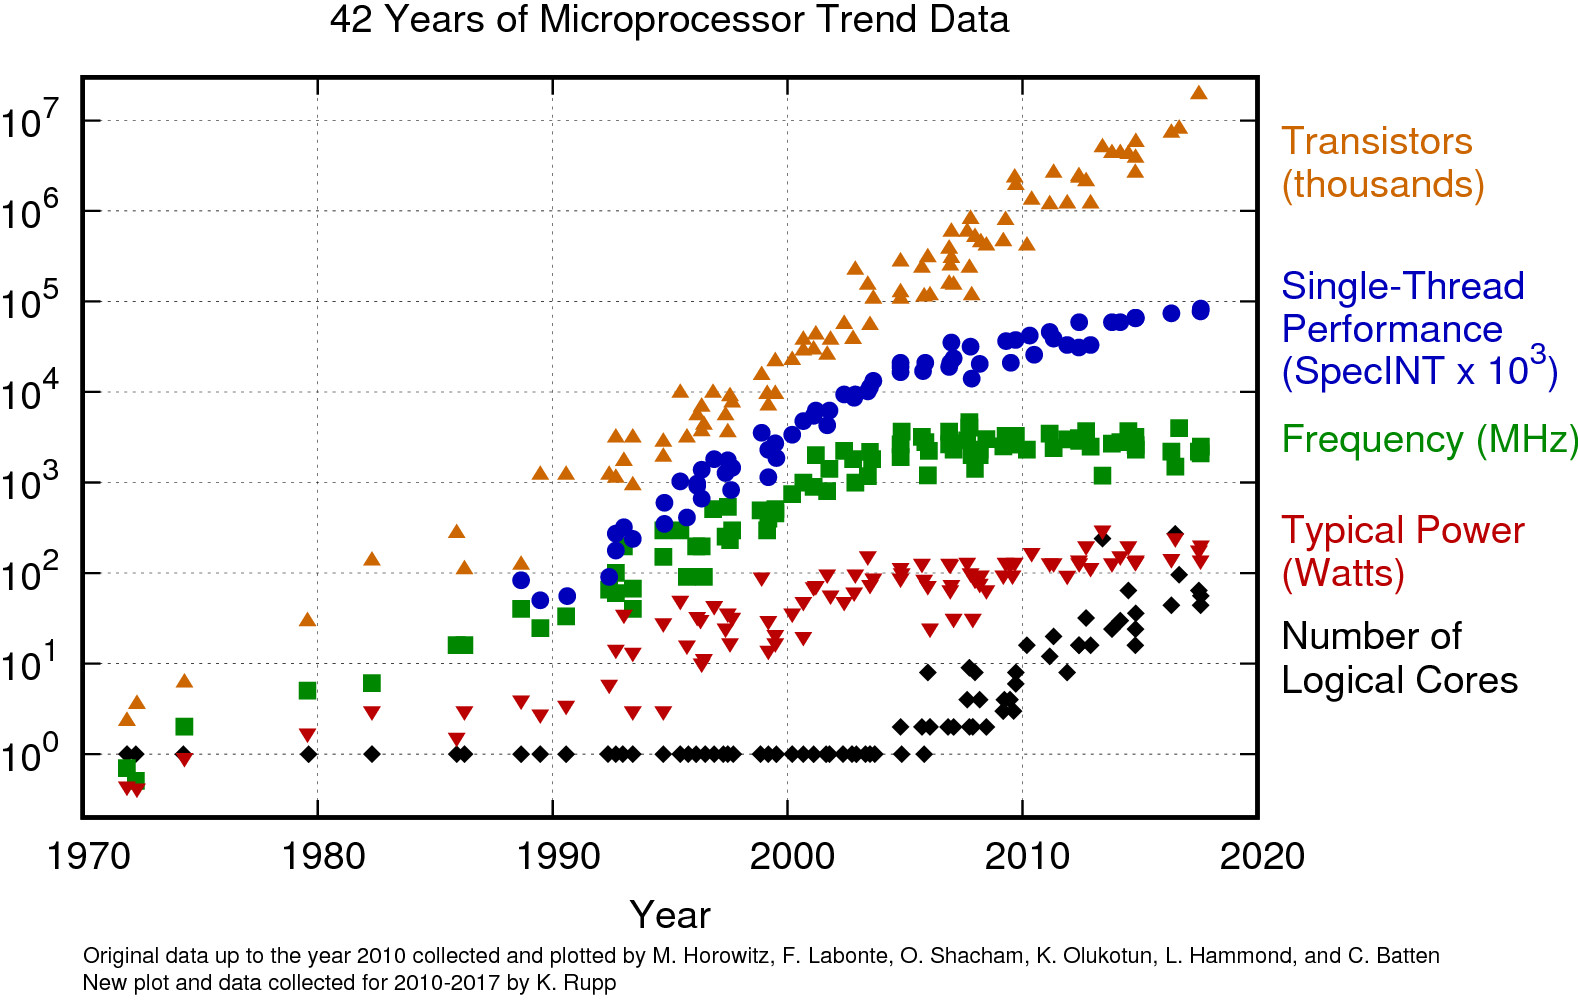
\includegraphics[width=\textwidth]{42-years-processor-trend.jpg}
\end{frame}

\begin{frame}
  \frametitle{La ``loi de Moore'' et la fin du ``\textit{Dennard Scaling}''}

  \framesubtitle{Repercussion sur le TOP500}
  
  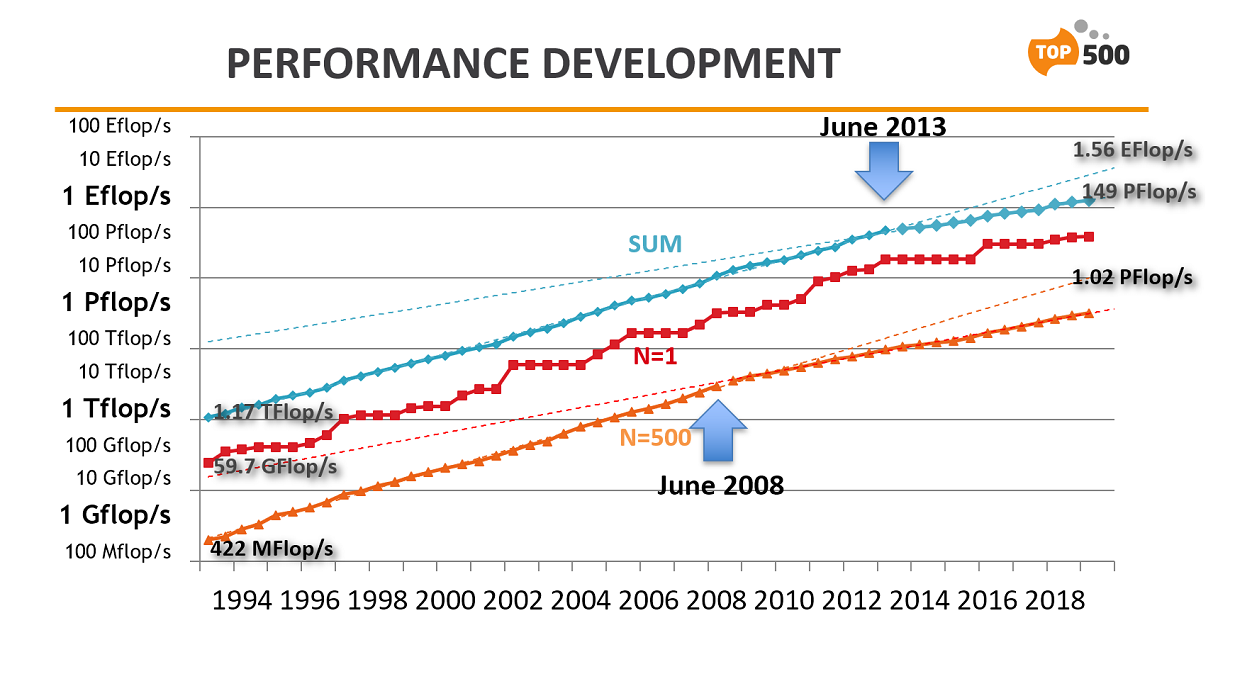
\includegraphics[width=\textwidth]{Top500-Dennard-scaling-effect.png}
\end{frame}

\begin{frame}
  \frametitle{Amélioration de l'efficacité énergétique (FLOP/Watt)}
  \framesubtitle{$\leadsto$ réduire fréquence, augmenter \# processeurs}

  \centering

  \small CPU = Cortex A9 (ARM, smartphone). Calcul = (morceau de la) FFT. 
  
  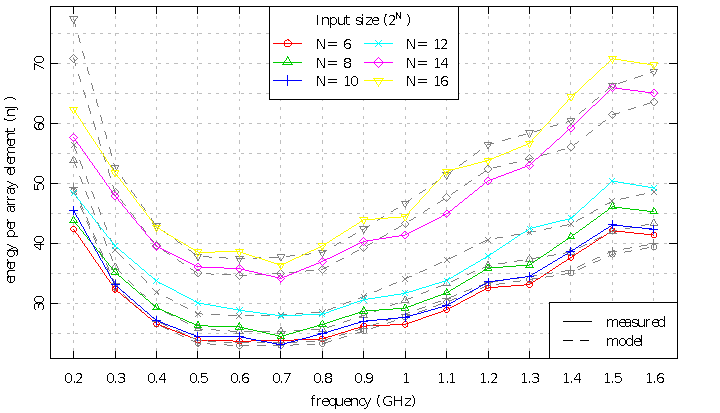
\includegraphics[width=\textwidth]{cpu_freq_scaling.pdf}
\end{frame}

%%%%%%%%%%%%%%%%%%%%%%%%%%%%%%%%%%%%%%%%%%%%%%%%%%%%%%%%%%%%%%%%%%%%%%

\begin{frame}
  \frametitle{Glossaire}

    \begin{description}
    \item[machine] ensemble des composants

    \item[\textit{cluster}] des serveurs de calcul réliés à un réseau (\sout{COVID})
      
    \item[noeud] un \og ordinateur\fg indépendant

    \item[baie] armoire contenants noeuds, switch, etc.

    \item[SMP] noeud qui contient plusieurs processeurs

    \item[processeur] objet qui contient au moins un \emph{coeur} + cache, etc.
  
    \item[\emph{socket}] prise sur laquelle on branche un processeur

    \item[coeur] circuit qui exécute du code de façon autonome

    \item[multicoeur] processeur qui contient plusieurs coeurs
  
    \item[thread matériel] contexte d'exécution autonome dans un coeur

    \item[SMT] coeur qui héberge plusieurs threads matériels
    \end{description}

\end{frame}

%%%%%%%%%%%%%%%%%%%%%%%%%%%%%%

\begin{frame}
  \frametitle{Glossaire --- difficulté avec \og \emph{thread}\fg}

  \begin{center}
    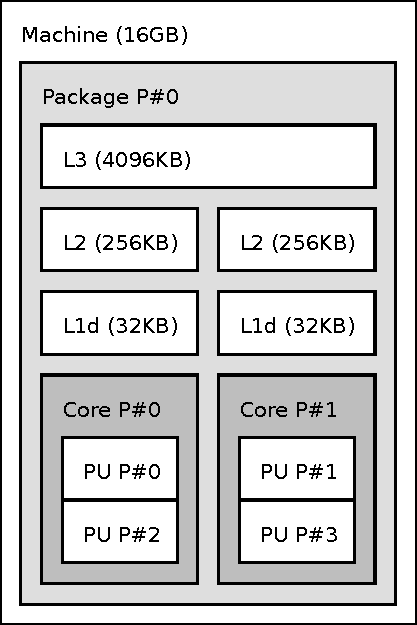
\includegraphics[height=6cm]{lstopo_laptop.pdf}%
    \quad \small sortie de \texttt{lstopo} sur un laptop
  \end{center}

  \begin{itemize}
  \item thread matériel $\neq$ thread logiciel (OS)
  \item ``coeur physique'' $\approx$ coeur
  \item ``coeur logique''  $\approx$ thread matériel
  \end{itemize}
  
\end{frame}

%%%%%%%%%%%%%%%%%%%%%%%%%%%%%%

\begin{frame}
  \frametitle{Notions de processus et de thread dans les OS}

\begin{description}
\item[Processus] \og flot d'exécution \fg $~+~$ \og espace mémoire \fg 
\item[Thread] \og flot d'exécution \fg 
\end{description}

\pause 

\bigskip

\centering

%% Tanenbaum sur les Systèmes d'exploitation : 
\begin{tabular}{c|c}
Eléments propres   & Eléments propres \\
à chaque processus & à chaque thread \\ 
\hline
Espace d'adressage & Compteur ordinal \\ 
Variables globales & Registres \\
Fichiers ouverts & Pile (dont variables locales)\\
  Processus enfant, signaux\dots & Etat \\
  \hline
  \\
    
\includegraphics[height=0.15\textheight]{multi-processus}$\quad$&
    
\includegraphics[height=0.15\textheight]{multi-thread} \\
    Mode multi-processus    &
    $\quad$ Mode multi-thread $\quad$ \\
\end{tabular}
\end{frame} 

%%%%%%%%%%%%%%%%%%%%%%%%%%%%%%%%%%%%%%%%%%%%%%%%%%%

\begin{frame}
\frametitle{Les machines parallèles --- classification}

\begin{block}{Classification de Flynn (1966) :}

  \begin{center}
    \begin{tabular}{|l|l|c|c|}
      \cline{3-4}
      \multicolumn{2}{c|}{}    & \multicolumn{2}{c|}{Flot de données} \\
      \cline{3-4}
      \multicolumn{2}{c|}{}    & unique & multiple \\
      \hline
      Flot           & unique   & \bf SISD   & \bf SIMD \\
      \cline{2-4}
      d'instructions & multiple & \bf MISD   & \bf MIMD \\
      \hline
    \end{tabular}
  \end{center}
\end{block}

\pause
  
  \begin{itemize}

  \item {\bf machines SISD} Ce sont les machines séquentielles !

  \item {\bf machines MISD} Ça n'existe pas vraiment.
    
    {\small \it (Chaque processeur recevrait des instructions distinctes opérant sur le même
    flot de données ???)}
  \end{itemize}

\end{frame}


%%%%%%%%%%%%%%%%%%%%%%%%%%%%%%%%%%%%%%%%%%%%%%%%%%%%%%%%%%%%%%%%%%%%%
\begin{frame}<1>[label=flynn_suite]
\frametitle{Classification de Flynn (suite)}

\begin{itemize}
  
\item {\bf machines SIMD} 

Les unités de traitement %% (processing units)  %% ou unités de calcul  
exécutent simultanément la même opération sur
leurs données propres.
\begin{itemize}
\item fonctionnement synchrone
\item une seule unité de contr\^ole centralisée 
\item exemples :
  \begin{itemize}
  \item machines vectorielles des années 1970--90 (CRAY , NEC \dots)
  \item instructions vectorielles (SSE, AVX2, AVX-512, NEON, \dots)
  \item Graphics Processing Units (GPUs)
  \end{itemize}
\end{itemize}


\item<2-> {\bf machines MIMD} 

Les processeurs peuvent effectuer différentes opérations sur
différentes données simultanément.
\begin{itemize}
\item fonctionnement asynchrone 
\item exemples :
  \begin{itemize}
  \item grappe ({\it cluster}) de PC
  \item Toutes les grosses machines de HPC    
  \end{itemize}
\end{itemize}

\end{itemize}
\end{frame}

%%%%%%%%%%%%%%%%%%%%%%%%%%%%%%%%%%%%%%%%%%%%%%%%%%%%%%%%%%%%%%%

\begin{frame}
\frametitle{SIMD}

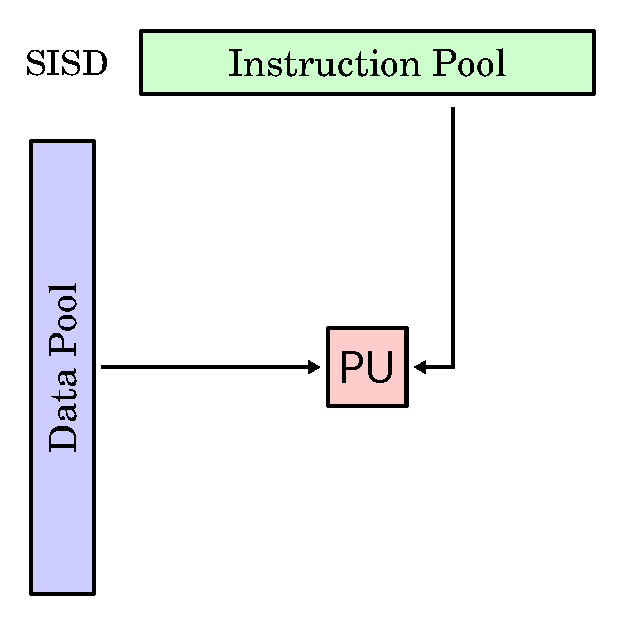
\includegraphics[width=0.4\textwidth]{SISD}
\hfill
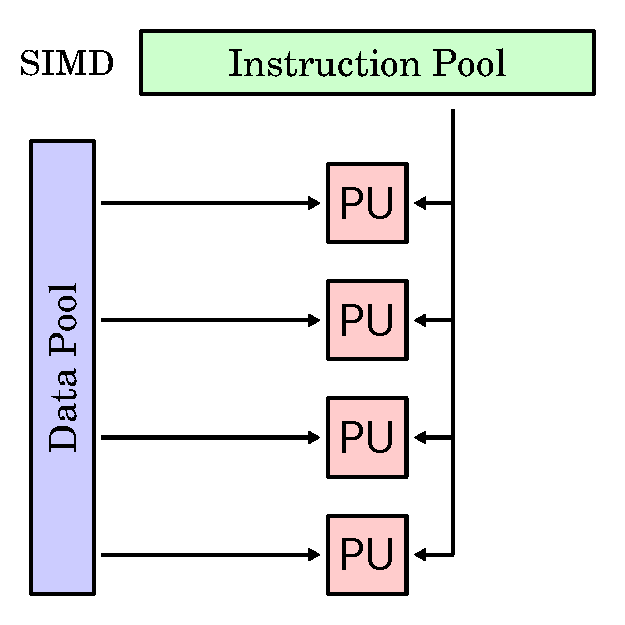
\includegraphics[width=0.4\textwidth]{SIMD}

\hfill (image: Wikipédia)

\end{frame}

%%%%%%%%%%%%%%%%%%%%%%%%%%%%%%%%%%%%%%%%%%%%%%%%%%%%%%%%%%%%%%%

\againframe<2>{flynn_suite}

%%%%%%%%%%%%%%%%%%%%%%%%%%%%%%%%%%%%%%%%%%%%%%%%%%%%%%%%%%%%%%%

\begin{frame}
  \frametitle{Mémoire distribuée}
  \framesubtitle{Classification selon l'organisation de la mémoire}

  \begin{center}
    \begin{tikzpicture}[scale=1.33,>=stealth]
      \node[draw, inner sep=3pt] (P0) at (0, 1)  {CPU};
      \node[draw, inner sep=3pt] (P1) at (1, 1)  {CPU};
      \node[draw, inner sep=3pt] (P2) at (2, 1)  {CPU};
      \node[draw, inner sep=3pt] (P3) at (3, 1)  {CPU};

      \node[draw, shape=circle, inner sep=1pt] (R0) at (0, 2.25)  {RAM};
      \node[draw, shape=circle, inner sep=1pt] (R1) at (1, 2.25)  {RAM};
      \node[draw, shape=circle, inner sep=1pt] (R2) at (2, 2.25)  {RAM};
      \node[draw, shape=circle, inner sep=1pt] (R3) at (3, 2.25)  {RAM};

      \filldraw[fill=LightGray] (-1, 0) rectangle node (net) {Réseau} +(5, -0.33);

      \draw[<->,thick] (P0) edge (0, 0) edge (R0);
      \draw[<->,thick] (P1) edge (1, 0) edge (R1);
      \draw[<->,thick] (P2) edge (2, 0) edge (R2);
      \draw[<->,thick] (P3) edge (3, 0) edge (R3);
    \end{tikzpicture}
  \end{center}

  \begin{itemize}
  \item Chaque processeur possède sa propre mémoire
    
  \item Communication $=$ échange de messages sur le réseau

  \item Performances du réseau = aspect \textbf{critique} de la machine
  \end{itemize}
\end{frame}

%%%%%%%%%%%%%%%%%%%%%%%%%%%%%%%%%%%%%%%%%%%%%%%%%%%%%%%%%%%%%%%%%%%%

\begin{frame}
  \frametitle{Mauvaise idée}
  \framesubtitle{réseau en arbre, switches quelconques}
  \begin{tikzpicture}
    \path[red, dotted, use as bounding box] (-0.5, 1) rectangle (10, -4.5);
    \node at(5, 0) (switch) {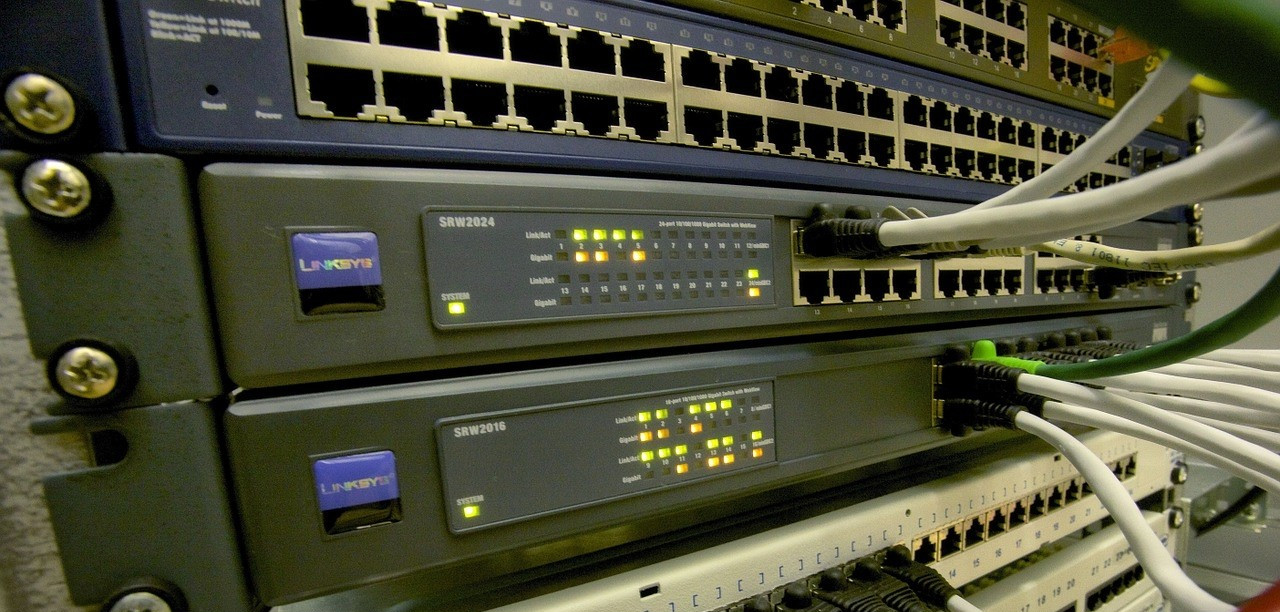
\includegraphics[width=5cm]{old_switch.jpg}};

    \foreach \i in {0, 1, 2, 3, 4, 5} {
      \path (\i*2cm, -3) node {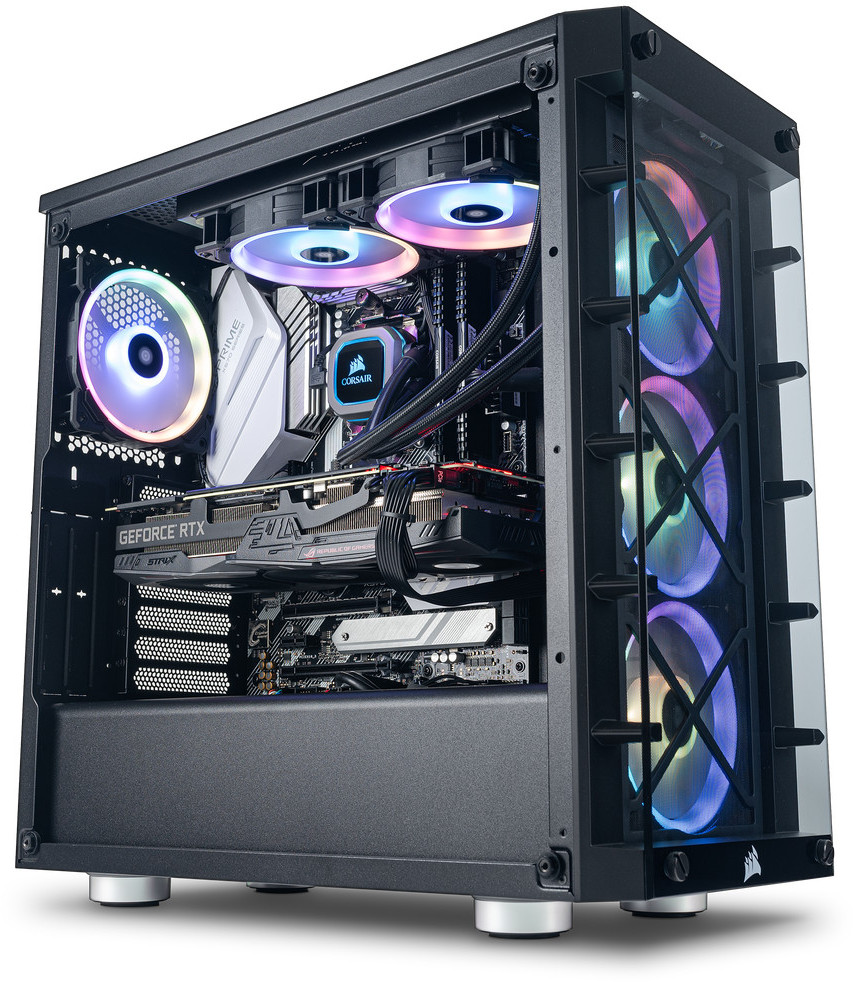
\includegraphics[width=2cm]{gamer.jpg}} edge[->] (switch);
    }
  \end{tikzpicture}

  \bigskip

  Mauvaises performances, problème de passage à l'échelle.
  
\end{frame}

%%%%%%%%%%%%%%%%%%%%%%%%%%%%%%%%%%%%%%%%%%%%%%%%%%%%%%%%%%%%%%%%%

\begin{frame}
  \frametitle{Topologie Réseau}
  \framesubtitle{Fat Tree (Infiniband)}

  \centering
  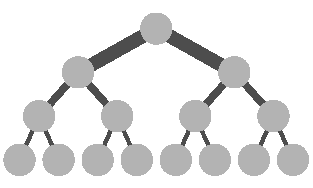
\includegraphics[width=10cm]{fat_tree.pdf}
\end{frame}

%%%%%%%%%%%%%%%%%%%%%%%%%%%%%%%%%%%%%%%%%%%%%%%%%%%%%%%%%%%%%%%

\begin{frame}
  \frametitle{Fat tree (2 levels)}
  
  \begin{tikzpicture}[scale=0.5]
  \draw[ultra thick] (-0.5, -0.5) rectangle (19.5, 4.5);
  \draw[dashed, thick] (10.5, 3.5) -- (12.5, 3.5);
  \draw[dashed, thick] (7.5, 0.5) -- (11.5, 0.5);
  
  \foreach \j / \lab in {3/1, 7/2, 13/{$R/2$}} {
    \begin{scope}[xshift=\j*1cm]
      \draw (0, 3) rectangle node {\lab} +(3, 1);
      \foreach \i in {1, 2, ..., 19} {
        \draw (0.15*\i, 3) -- +(0, -0.1);
      }
    \end{scope}
  }

  \foreach \j / \lab in {0/1, 4/2, 12/{$R-1$}, 16/{$R$}} {
    \begin{scope}[xshift=\j*1cm]
      \draw (0, 0) rectangle node {\lab} +(3, 1);
      \foreach \i in {1, 2, ..., 9} {
        \draw (0.3*\i, 0) -- +(0, -1);
        \draw (0.3*\i, 1) -- +(0, 0.1);
      }
    \end{scope}
  }

  \draw (0 + 0.3*1, 1.1) -- (3 + 0.15*1, 2.9);
  \draw (0 + 0.3*2, 1.1) -- (7 + 0.15*1, 2.9);
  \draw (0 + 0.3*9, 1.1) -- (13 + 0.15*1, 2.9);

  \draw (4 + 0.3*1, 1.1) -- (3 + 0.15*2, 2.9);
  \draw (4 + 0.3*2, 1.1) -- (7 + 0.15*2, 2.9);
  \draw (4 + 0.3*9, 1.1) -- (13 + 0.15*2, 2.9);

  \draw (12 + 0.3*1, 1.1) -- (3 + 0.15*18, 2.9);
  \draw (12 + 0.3*2, 1.1) -- (7 + 0.15*18, 2.9);
  \draw (12 + 0.3*9, 1.1) -- (13 + 0.15*18, 2.9);

  \draw (16 + 0.3*1, 1.1) -- (3 + 0.15*19, 2.9);
  \draw (16 + 0.3*2, 1.1) -- (7 + 0.15*19, 2.9);
  \draw (16 + 0.3*9, 1.1) -- (13 + 0.15*19, 2.9);
\end{tikzpicture}

\bigskip

\begin{itemize}
\item Switches \textbf{non-bloquants}
\item Un switch à $R^2 / 2$ ports à partir de $1.5R$ switches à $R$ ports
\item Infiniband : $R = 36 \leadsto $ 648 ports
\end{itemize}

\end{frame}

%%%%%%%%%%%%%%%%%%%%%%%%%%%%%%%%%%%%%%%%%%%%%%%%%%%%%%%%%%%%

\begin{frame}
  \frametitle{Switch infiniband à 648 ports...}
  \centering
  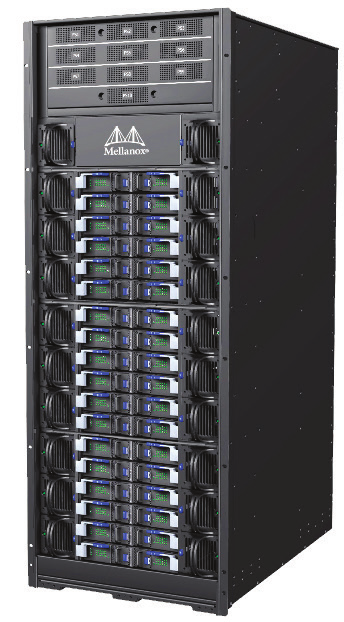
\includegraphics[height=0.75\textheight]{infiniband.png}
\end{frame}

%%%%%%%%%%%%%%%%%%%%%%%%%%%%%%%%%%%%%%%%%%%%%%%%%%%%%%%%%%%%%

\begin{frame}
  \frametitle{Fat tree (3 levels)}
  \begin{tikzpicture}[scale=0.5]
   \draw[ultra thick] (-0.5, -0.5) rectangle (21.5, 5.5);
   \draw[dashed, thick] (12.5, 4) -- (14.5, 4);
   \draw[dashed, thick] (11.5, 0.5) -- (13.5, 0.5);
  
  \foreach \j / \lab in {3/1, 8/2, 15/{$R/2$}} {
    \begin{scope}[xshift=\j*1cm]
      \draw[fill=gray!30, thick] (0, 3) rectangle node {\lab} +(4, 2);
      \foreach \i in {1, 2, ..., 39} {
        \draw (0.1*\i, 3) -- +(0, -0.2);
      }
    \end{scope}
  }

  \foreach \j / \lab in {0/1, 4/2, 8/3, 14/{$R^2/2-1$}, 18/{$R^2/2$}} {
    \begin{scope}[xshift=\j*1cm]
      \draw (0, 0) rectangle node {\lab} +(3, 1);
      \foreach \i in {1, 2, ..., 9} {
        \draw (0.3*\i, 0) -- +(0, -1);
        \draw (0.3*\i, 1) -- +(0, 0.2);
      }
    \end{scope}
  }

  \draw (0 + 0.3*1, 1.2) -- (3 + 0.1*1, 2.8);
  \draw (0 + 0.3*2, 1.2) -- (8 + 0.1*1, 2.8);
  \draw (0 + 0.3*9, 1.2) -- (15 + 0.1*1, 2.8);

  \draw (4 + 0.3*1, 1.2) -- (3 + 0.1*2, 2.8);
  \draw (4 + 0.3*2, 1.2) -- (8 + 0.1*2, 2.8);
  \draw (4 + 0.3*9, 1.2) -- (15 + 0.1*2, 2.8);

  \draw (8 + 0.3*1, 1.2) -- (3 + 0.1*3, 2.8);
  \draw (8 + 0.3*2, 1.2) -- (8 + 0.1*3, 2.8);
  \draw (8 + 0.3*9, 1.2) -- (15 + 0.1*3, 2.8);

  
  \draw (14 + 0.3*1, 1.2) -- (3 + 0.1*38, 2.8);
  \draw (14 + 0.3*2, 1.2) -- (8 + 0.1*38, 2.8);
  \draw (14 + 0.3*9, 1.2) -- (15 + 0.1*38, 2.8);

  \draw (18 + 0.3*1, 1.2) -- (3 + 0.1*39, 2.8);
  \draw (18 + 0.3*2, 1.2) -- (8 + 0.1*39, 2.8);
  \draw (18 + 0.3*9, 1.2) -- (15 + 0.1*39, 2.8);
\end{tikzpicture}

\bigskip


\begin{itemize}
\item Même technique en utilisant la construction précédente
\item $R^3 / 4$ ports avec $1.25 R^2$ switches à $R$ ports
\item Infiniband : $R = 36 \leadsto 11 644$ ports
\item Utilisé dans \texttt{Summit} avec 9216 CPUs (un peu de marge)
  \begin{itemize}
  \item 1 baie = 18 noeuds = 36 CPUs = 36 interfaces réseaux
  \item 2 switches 36 ports par baie
  \item 256 baies
  \end{itemize}
\end{itemize}
\end{frame}

%%%%%%%%%%%%%%%%%%%%%%%%%%%%%%%%%%%%%%%%%%%%%%%%%%%%%%%%%%%%%%

\begin{frame}
  \frametitle{Fat tree --- coût élevé du cablage}
  \framesubtitle{Au final, ça ressemble à ça}

  \centering
  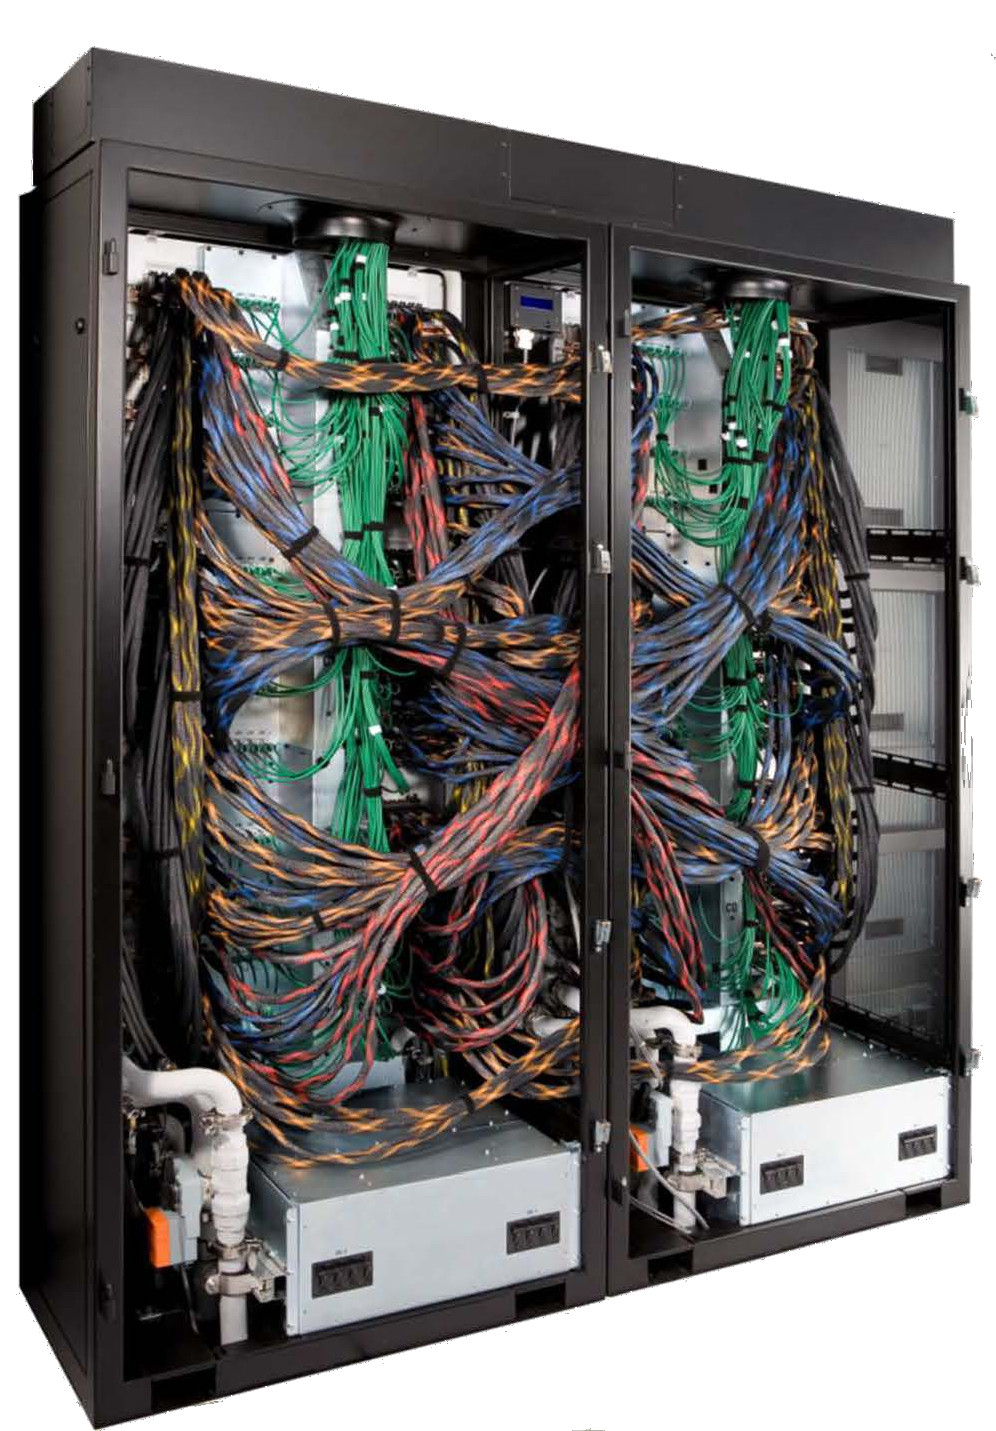
\includegraphics[height=8cm]{wiring}

  \bigskip

  Longueur de cable $\geq N^{1.5}$.
\end{frame}


%%%%%%%%%%%%%%%%%%%%%%%%%%%%%%%%%%%%%%%%%%%%%%%%%%%%%%%%%%%%%%%

\begin{frame}
  \frametitle{Topologie Réseau}
  \framesubtitle{Tore 3D (IBM BlueGene/P, Cray XT3, ...)}

  \begin{center}
    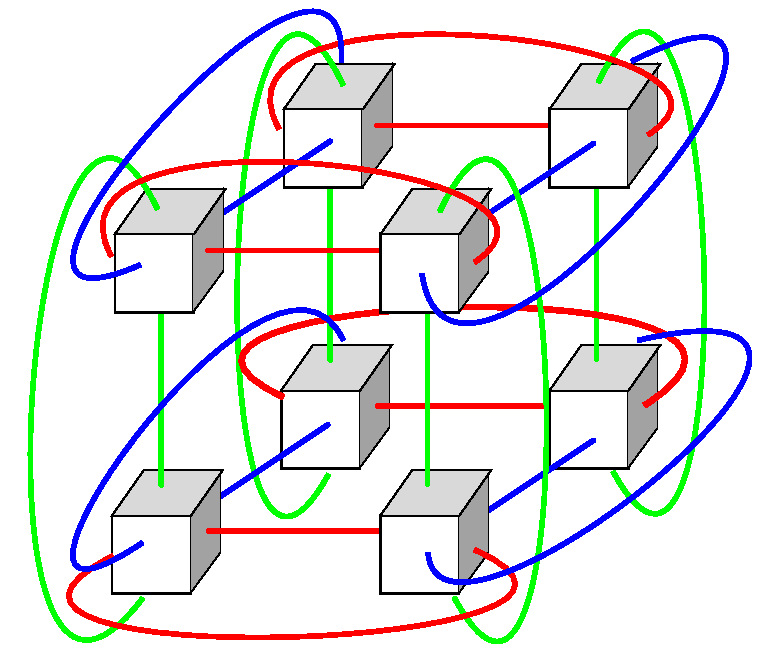
\includegraphics[height=6cm]{2x2x2torus.pdf}
  \end{center}

  \begin{itemize}
  \item Longueur de cable proportionnelle à \#CPU
  \item Utilisé sur de très grandes machines (e.g. $48 \times 72 \times 24$)
  \end{itemize}
  
\end{frame}


\begin{frame}
  \frametitle{Topologie Réseau}
  \framesubtitle{Tore 5D (IBM BlueGene/Q)}

  \centering
  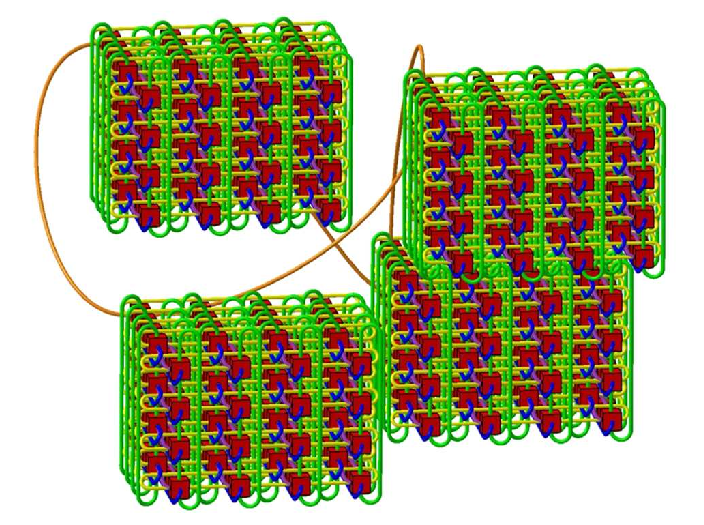
\includegraphics[height=8cm]{5D_torus.pdf}
\end{frame}

\begin{frame}
  \frametitle{Topologie Réseau}
  \framesubtitle{Dragonfly (Cray \og Aries\fg interconnect)}

  \centering
  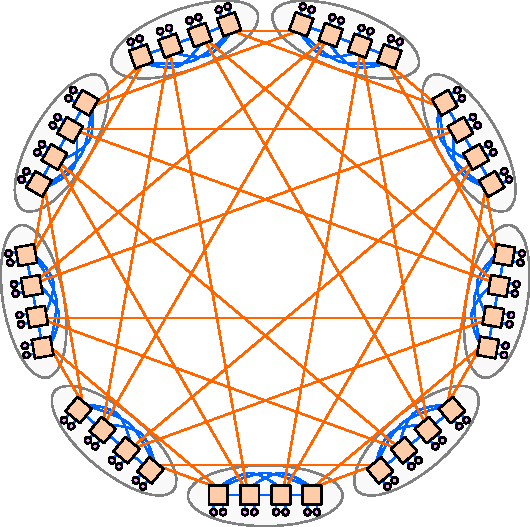
\includegraphics[height=8cm]{dragonfly.pdf}
\end{frame}



%%%%%%%%%%%%%%%%%%%%%%%%%%%%%%%%%%%%%%%%%%%%%%%%%%%%%%%%%%%%%%%%%%%%%

\begin{frame}
  \frametitle{Mémoire partagée}
  \framesubtitle{Classification selon l'organisation de la mémoire}

  \begin{center}
    \begin{tikzpicture}[scale=1.33,>=stealth]
      \node[draw, inner sep=3pt] (P0) at (0, 1)  {CPU};
      \node[draw, inner sep=3pt] (P1) at (1, 1)  {CPU};
      \node[draw, inner sep=3pt] (P2) at (2, 1)  {CPU};
      \node[draw, inner sep=3pt] (P3) at (3, 1)  {CPU};

      \node[draw, shape=circle, inner sep=5pt] (R0) at (6, -0.33/2)  {RAM};

      \filldraw[fill=LightGray] (-1, 0) rectangle node (net) {Bus mémoire} +(5, -0.33);

      \draw[<->,thick] (P0) edge (0, 0);
      \draw[<->,thick] (P1) edge (1, 0);
      \draw[<->,thick] (P2) edge (2, 0);
      \draw[<->,thick] (P3) edge (3, 0);
      
      \draw[<->,thick] (R0) edge (4, -0.33 / 2);
    \end{tikzpicture}
  \end{center}

  
  \begin{itemize}
    
  \item CPUs reliés à l'ensemble de la mémoire par un bus.
    
  \item Chacun peut accéder à l'intégralité de la mémoire.
    
  \item Communications $\leftrightarrow $ lecture/écriture en mémoire.    
  \end{itemize}

  \bigskip
  \begin{itemize}
  \item Attention aux conflits d'accès à une même adresse !
  \end{itemize}  
\end{frame}

%%%%%%%%%%%%%%%%%%%%%%%%%%%%%%%%%%%%%%%%%%%%%%%%%%%%%%%%%%%%%%%%

%%%%%%%%%%%%%%%%%%%%%%%%%%%%%%%%%%%%%%%%%%%%%%%%%%%%%%%%%%%%%%%%%%%%%
\begin{frame}
  \frametitle{Mémoire partagée}
  \framesubtitle{Classification selon l'organisation de la mémoire}


  \begin{block}{{\it Race condition :}}
    Il y a {\it race condition} lorsque  
    \begin{itemize}
    \item au moins 2 processeurs accèdent à la même variable
    \item au moins un processeur y accède en écriture 
    \item ces accès sont potentiellement concurrents (ils peuvent
      être effectués \og au même moment \fg)
    \end{itemize}
  \end{block}
  
  \medskip
  
  \mintinline{C}{i = i + 1;}
  
  \medskip
  
  \begin{exampleblock}{Solution}
    mécanismes de synchronisation (section critique,
    opération atomique, barrière de synchronisation)
  \end{exampleblock}
\end{frame}


%%%%%%%%%%%%%%%%%%%%%%%%%%%%%%%%%%%%%%%%%%%%%%%%%%%%%%%%%%%%%%%%%

\begin{frame}
  \frametitle{Non-Uniform Memory Access}
  \framesubtitle{Classification selon l'organisation de la mémoire}

  \begin{alertblock}{Mémoire partagée : problème de passage à l'échelle}
    Contention sur le bus mémoire...
  \end{alertblock}

  \begin{exampleblock}{Solution}
    \begin{itemize}
    \item Simuler mémoire partagée avec mémoire distribuée.
    \item Chaque CPU \og contrôle\fg une partie de la mémoire.
      \begin{itemize}
      \item Il y accède \emph{directement}
      \end{itemize}
    \item Pour accéder au reste de la mémoire, il faut passer par les autres
      CPUs.
    \item[$\Rightarrow$] Réseau \textit{ad hoc}, très rapide.
    \end{itemize}
  \end{exampleblock}
\end{frame}

%%%%%%%%%%%%%%%%%%%%%%%%%%%%%%%%%%%%%%%%%%%%%%%%%%%

\begin{frame}
  \frametitle{Non-Uniform Memory Access}
  \framesubtitle{Un vrai exemple}

  \begin{itemize}
  \item un noeud SMP avec $2 \times$ CPU AMD EYPC \og Naples\fg
  \item 4 $\times$ contrôleurs RAM indépendants par CPU
  \item<3-> Graphe complet à l'intérieur d'un CPU
  \item<4-> Interconnection partielle entre les 2 sockets
  \item<4-> Lien rouge = $\approx 2\times$ plus de latence
  \end{itemize}

  \medskip

    \begin{center}
      \begin{tikzpicture}[scale=1.33,>=stealth]
        \path[use as bounding box] (-3, -2.25) rectangle +(6, 4);
        \node at (0, -0.15) {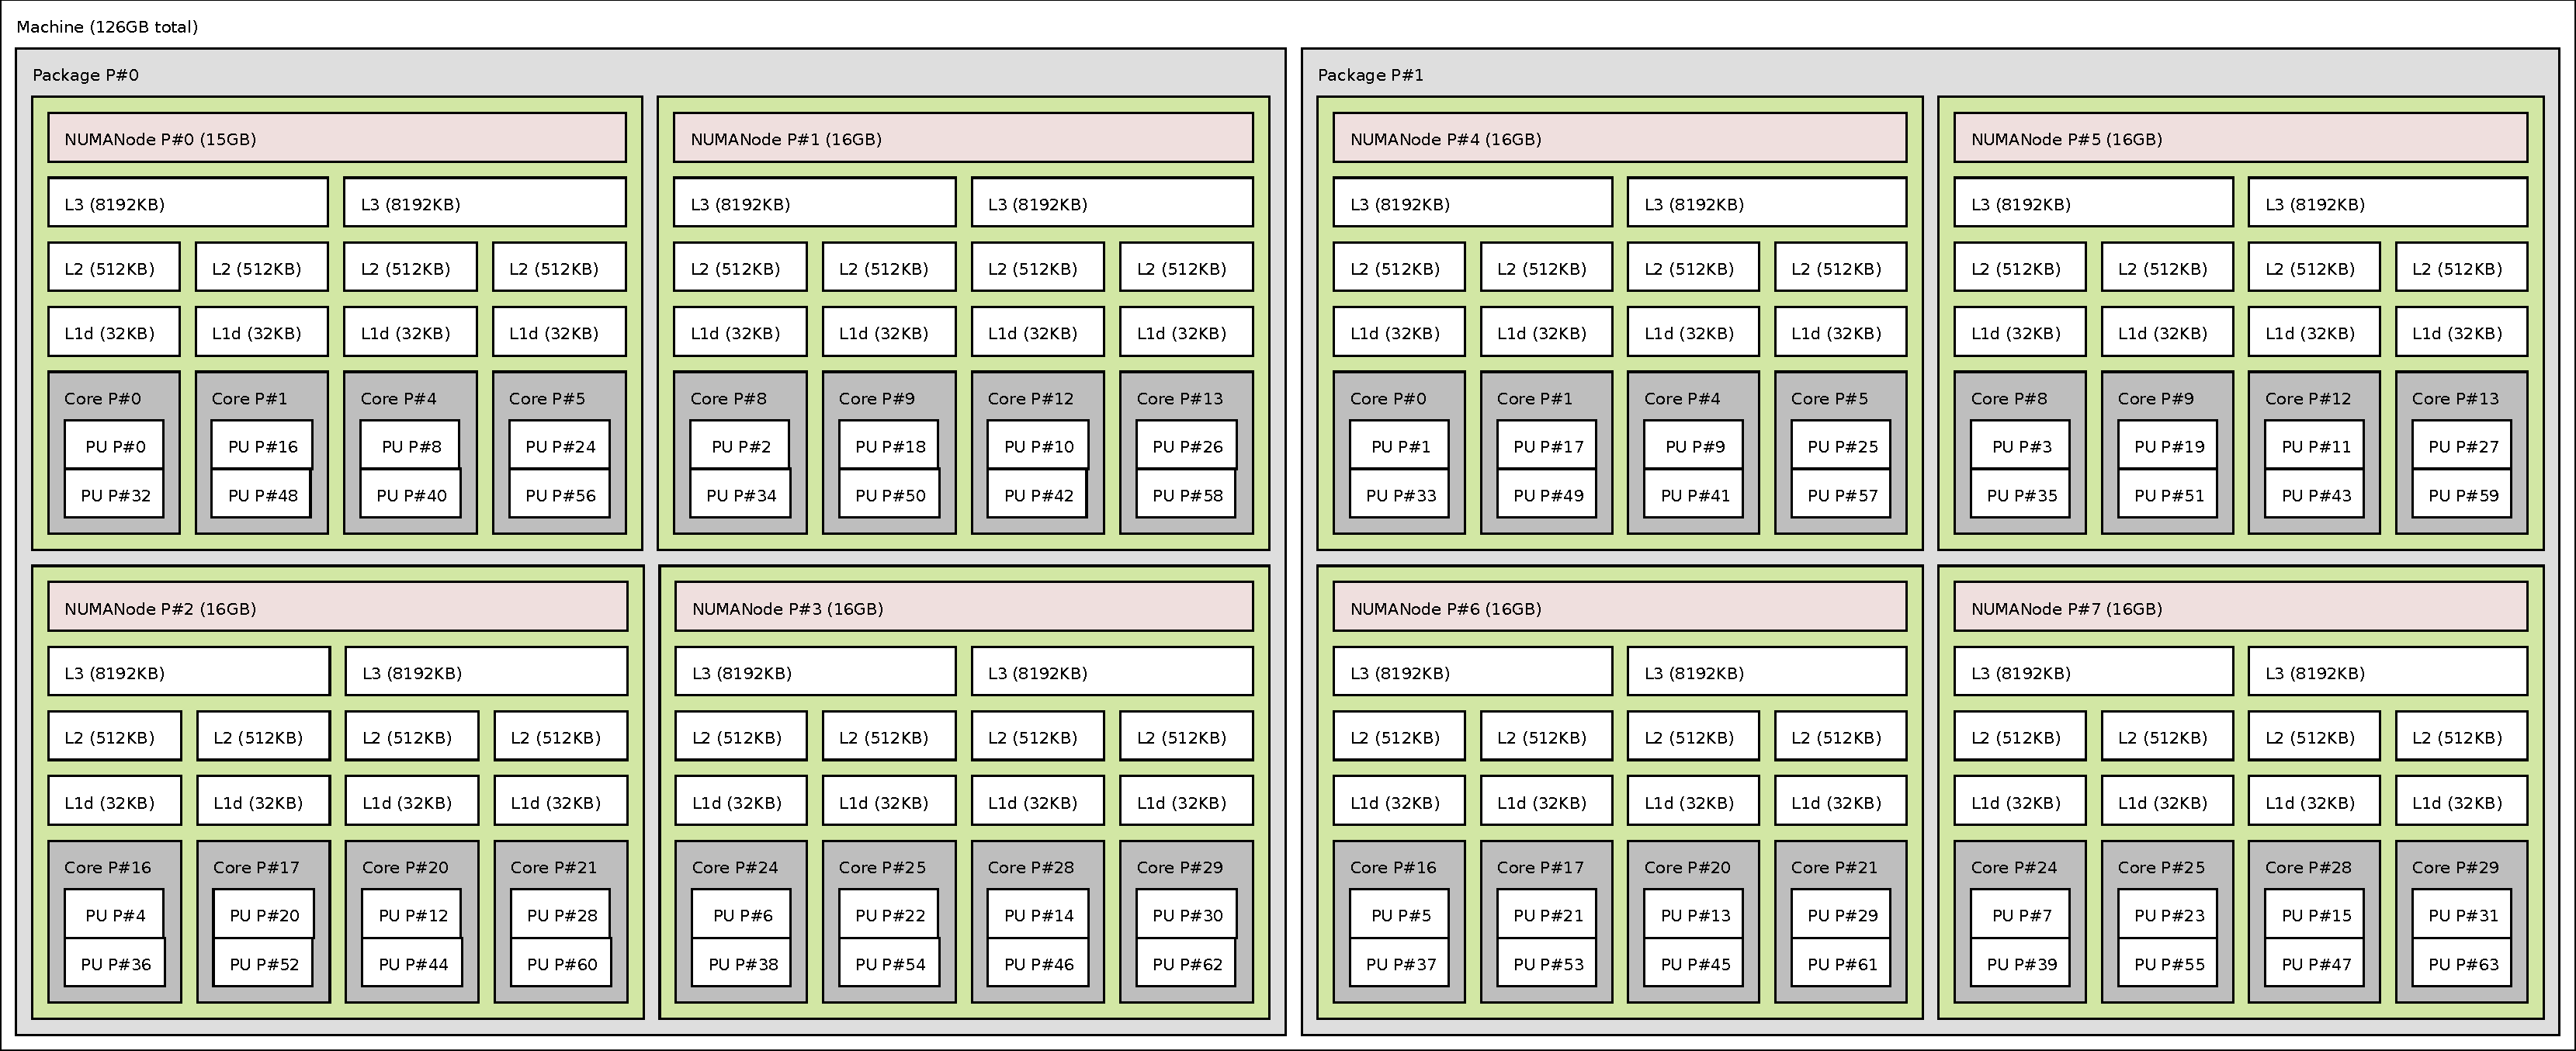
\includegraphics[width=\textwidth]{lstopo_chiclet}};
        
        \node<2->[draw, ultra thick, fill=white, inner sep=5pt] (P2) at (-3, -1)  {$P_2$};
        \node<2->[draw, ultra thick, fill=white, inner sep=5pt] (P0) at (-3, 0.5)  {$P_0$};
        \node<2->[draw, ultra thick, fill=white, inner sep=5pt] (P3) at (-1, -1)  {$P_3$};
        \node<2->[draw, ultra thick, fill=white, inner sep=5pt] (P1) at (-1, 0.5)  {$P_1$};
        \node<2->[draw, ultra thick, fill=white, inner sep=5pt] (P6) at (1, -1)  {$P_6$};
        \node<2->[draw, ultra thick, fill=white, inner sep=5pt] (P4) at (1, 0.5)  {$P_4$};
        \node<2->[draw, ultra thick, fill=white, inner sep=5pt] (P7) at (3, -1)  {$P_7$};
        \node<2->[draw, ultra thick, fill=white, inner sep=5pt] (P5) at (3, 0.5)  {$P_5$};

        \node<2->[draw, shape=circle,ultra thick, fill=white, inner sep=1pt] (M2) at (-3.25, -2)  {$M_2$};
        \node<2->[draw, shape=circle,ultra thick, fill=white, inner sep=1pt] (M0) at (-3.25, 1.5)  {$M_0$};
        \node<2->[draw, shape=circle,ultra thick, fill=white, inner sep=1pt] (M3) at (-1.25, -2)  {$M_3$};
        \node<2->[draw, shape=circle,ultra thick, fill=white, inner sep=1pt] (M1) at (-1.25, 1.5)  {$M_1$};
        \node<2->[draw, shape=circle,ultra thick, fill=white, inner sep=1pt] (M6) at (1.25, -2)  {$M_6$};
        \node<2->[draw, shape=circle,ultra thick, fill=white, inner sep=1pt] (M4) at (1.25, 1.5)  {$M_4$};
        \node<2->[draw, shape=circle,ultra thick, fill=white, inner sep=1pt] (M7) at (3.25, -2)  {$M_7$};
        \node<2->[draw, shape=circle,ultra thick, fill=white, inner sep=1pt] (M5) at (3.25, 1.5)  {$M_5$};

        \draw<3->[ultra thick,<->] (P0) edge (P1) edge (P2) edge (P3);
        \draw<3->[ultra thick,<->] (P1) edge (P2) edge (P3);
        \draw<3->[ultra thick,<->] (P2) edge (P3);
        \draw<3->[ultra thick,<->] (P4) edge (P5) edge (P6) edge (P7);
        \draw<3->[ultra thick,<->] (P5) edge (P6) edge (P7);
        \draw<3->[ultra thick,<->] (P6) edge (P7);
        \draw<4>[ultra thick,red,<->] (P2) edge[bend right=2cm] (P4);
        \draw<4>[ultra thick,red,<->] (P3) edge[bend left=2cm] (P5);
        \draw<4>[ultra thick,red,<->] (P0) edge[bend right=2cm] (P6);
        \draw<4>[ultra thick,red,<->] (P1) edge[bend left=2cm] (P7);

        \draw<2->[ultra thick,dotted] (P0) edge (M0);
        \draw<2->[ultra thick,dotted] (P1) edge (M1);
        \draw<2->[ultra thick,dotted] (P2) edge (M2);
        \draw<2->[ultra thick,dotted] (P3) edge (M3);
        \draw<2->[ultra thick,dotted] (P4) edge (M4);
        \draw<2->[ultra thick,dotted] (P5) edge (M5);
        \draw<2->[ultra thick,dotted] (P6) edge (M6);
        \draw<2->[ultra thick,dotted] (P7) edge (M7);
        
      \end{tikzpicture}
  \end{center}
\end{frame}

%%%%%%%%%%%%%%%%%%%%%%%%%%%%%%%%%%%%%%%%%%%%%%%%%%%

\begin{frame}
  \frametitle{En pratique...}

  \begin{itemize}
  \item machine = noeuds reliés par un réseau
    \begin{itemize}
      \item MIMD / mémoire \emph{distribuée}
    \end{itemize}
    \medskip
  \item Un noeud = plusieurs processeurs
    \begin{itemize}
    \item Sûrement NUMA
    \end{itemize}
    \medskip
  \item Dans un noeud = tous les coeurs ont accès à la RAM
    \begin{itemize}
    \item Mémoire \emph{partagée}
    \end{itemize}
    \medskip
  \item Dans un coeur = instructions vectorielles
    \begin{itemize}
    \item SIMD
    \end{itemize}
  \end{itemize}

  \bigskip

  Bref, on a droit à tout à la fois.
\end{frame}

%%%%%%%%%%%%%%%%%%%%%%%%%%%%%%%%%%%%%%%%%%%%%%%%%%%%%%%%

\begin{frame}[fragile]
  \frametitle{Instruction-Level Parallelism (ILP)}

  \begin{columns}
    \begin{column}{3cm}  
\begin{minted}{gas}
slwi 10,9,3
add 8,11,10
lwzx 10,11,10
lwz 7,4(8)
or. 10,10,7
bne 0,.L146
addi 5,5,8
stw 3,0(8)
stw 4,4(8)
cmplw 7,6,5
bne 7,.L24
lwz 9,144(19)
li 10,1
stw 10,20704(31)
addi 9,9,1
\end{minted}
%stw 9,144(19)
    \end{column}  

    \begin{column}{7cm}
      code = liste \emph{ordonnée} d'instructions

      \medskip

      \begin{alertblock}{Parallélisme au sein d'un coeur}
      \begin{itemize}
      \item \emph{Pipeline(s)}
      \item \emph{Superscalarité}
      \item \emph{Out-of-order execution}
      \item \emph{Simultaneous Multi-Threading}
      \end{itemize}
    \end{alertblock}

    \begin{itemize}
    \item[$\Rightarrow$] Mécanismes parallèles
    \item[$\Rightarrow$] Sémantique séquentielle
    \end{itemize}
    
    \end{column}
  \end{columns}
\end{frame}

%%%%%%%%%%%%%%%%%%%%%%%%%%%%%%%%%%%%%%%%%%%%%%%%%%%%%%%%%%%%%%%%%%%%%

\begin{frame}[fragile]
  \frametitle{Comment écrire des programmes parallèles ?}

  \begin{itemize}
  \item<1-> Parallélisation automatique
  \item<2-> \og Annotations\fg de parallélisme dans des programmes C (\red{OpenMP}, OpenACC)
  \item<3-> plain C + bibliothèques (\texttt{pthread}, \red{MPI})
  \item<4-> Nouveaux langages ?
  \end{itemize}

  \medskip

  \begin{overlayarea}{\textwidth}{5cm}
  \begin{block}<only@2>{OpenMP}
\begin{minted}{C}
#pragma omp parallel for
for (int i = 0; i < n; i++)
    for (int j = 0; j < n; j++)
        for (int k = 0; k < n; k++)
            C[i][j] += A[i][k] * B[k][j];
\end{minted}
  \end{block}


  \begin{block}<only@3>{Librairies}
\begin{minted}[fontsize=\scriptsize]{C}
 for(int t=0; t<NUM_THREADS; t++)
       pthread_create(&threads[t], NULL, ThreadFunction, (void *) t);
...
pthread_exit();
\end{minted}
  \end{block}

  \begin{block}<only@4>{Nouveaux langages (Go, UPC, coarray Fortran, ....)}
\begin{minted}[fontsize=\small]{go}
func main() {
    s := []int{7, 2, 8, -9, 4, 0}
    c := make(chan int)
    go sum(s[:len(s)/2], c)
    go sum(s[len(s)/2:], c)
    x, y := <-c, <-c
    fmt.Println(x, y, x+y)
}
\end{minted}
  \end{block}
\end{overlayarea}
\end{frame}


%%%%%%%%%%%%%%%%%%%%%%%%%%%%%%%%%%%%%%%%%%%%%%%%%%%%%%%%%%%%%%%%%%%%% 


\begin{frame}[fragile]
  \frametitle{Recycler les langages séquentiels}


  \begin{block}{\emph{Single Program Mutiple Data}}
    \begin{itemize}
    \item Même code séquentiel exécuté plusieurs fois en parallèle
    \item Variable spéciale : \texttt{rank}
    \item $\texttt{rank} = i$ sur le $i$-ème processeur
    \end{itemize}
  \end{block}

  \medskip
  
  \begin{minted}{C}
int i = rank;                /* data parallelism */
for (int j = 0; j < n; j++)
    for (int k = 0; k < n; k++)
        C[i][j] += A[i][k] * B[k][j];

if (rank == 0) {             /* control parallelism */
  <<Portion purement séquentielle>>
} else {
  <<Attend>>
}
\end{minted}
\end{frame}

%%%%%%%%%%%%%%%%%%%%%%%%%%%%%%%%%%%%%%%%%%%%%%%%%%%%%%%%%%%%%%%%%%

%%%%%%%%%%%%%%%%%%%%%%%%%%%%%%%%%%%%%%%%%%%%%%%%%%%%%%%%%%%%%%%%%%%%

\begin{frame}
\frametitle{Évaluation des performances}
\framesubtitle{Étudier le passage à l'échelle (\emph{scalability}) d'un algorithme parallèle}

Juge de paix : \alert{horloge murale}

\medskip

\begin{itemize}
\item $T_1(n)$ : temps nécessaire à l'exécution du \textbf{meilleur} algorithme
  séquentiel pour résoudre une instance de problème de taille $n$

  \medskip
  
\item $T_p(n)$ : temps nécessaire à l'exécution de l'algorithme parallèle
  considéré pour résoudre une instance de problème de taille $n$ avec $p$
  processeurs
\end{itemize}

\vspace*{-0.5cm}
\begin{columns}[t]

\column{0.5\textwidth}
\begin{block}{\textbf{Accélération}, \emph{speedup}}
  \[
    S(n,p)  =  \frac{T_1(n)}{T_p(n)}
  \]
\end{block}

\column{0.5\textwidth}
\begin{block}{{\bf Efficacité}, {\it efficiency}}
  \[
    E(n,p)  = \frac{S(n,p)}{p}
  \]
\end{block}
\end{columns}
\end{frame}


%%%%%%%%%%%%%%%%%%%%%%%%%%%%%%%%%%%%%%%%%%%%%%%%%%%%%%%%%%%%%%%%%%%%%
\begin{frame}
\frametitle{\emph{Strong scaling} (\og extensibilité forte \fg)}

\begin{alertblock}{Objectif de la parallélisation}
  \begin{itemize}
  \item Etude des performances en fonction de $p$ avec $n$ fixé
  \item Résoudre un problème de taille fixe le plus vite possible
  \end{itemize}
\end{alertblock}

\medskip

\begin{itemize} 
\item  {\bf Accélération linéaire ($\rightarrow$ l'idéal) :} 
les processeurs sont occupés à 100\% 
\[S(n,p)  = p \qquad E(n,p)  = 1\]

\medskip

\item {\bf Accélération sublinéaire :}
les processeurs sont occupés à moins de~100\% 

\medskip

\item {\bf Accélération supralinéaire :} difficile à envisager.
Toutefois cela peut arriver si la mémoire est mieux utilisée
(utilisation des caches), ou si l'on économise des calculs


\end{itemize}
\end{frame}




%%%%%%%%%%%%%%%%%%%%%%%%%%%%%%%%%%%%%%%%%%%%%%%%%%%%%%%%%%%%%%%%%%%%%
\begin{frame}
  \frametitle{\emph{Strong scaling}}
  \framesubtitle{Exemple d'une application non triviale}
  
  \begin{columns}
    \begin{column}{0.4\textwidth}
      \begin{center}
        \begin{tikzpicture}
          \path[use as bounding box] (-0.2, -0.5) rectangle +(4.2, 4.8);
          \draw[thick,->] (-0.15, 0.075) -- node[above,sloped] {Temps} +(0, 4.7);
          \draw[thick,->] (0, -0.15) -- node[below] {Processeurs} +(4.3, 0);
          \node[anchor=south west,inner sep=0] at (0, 0) {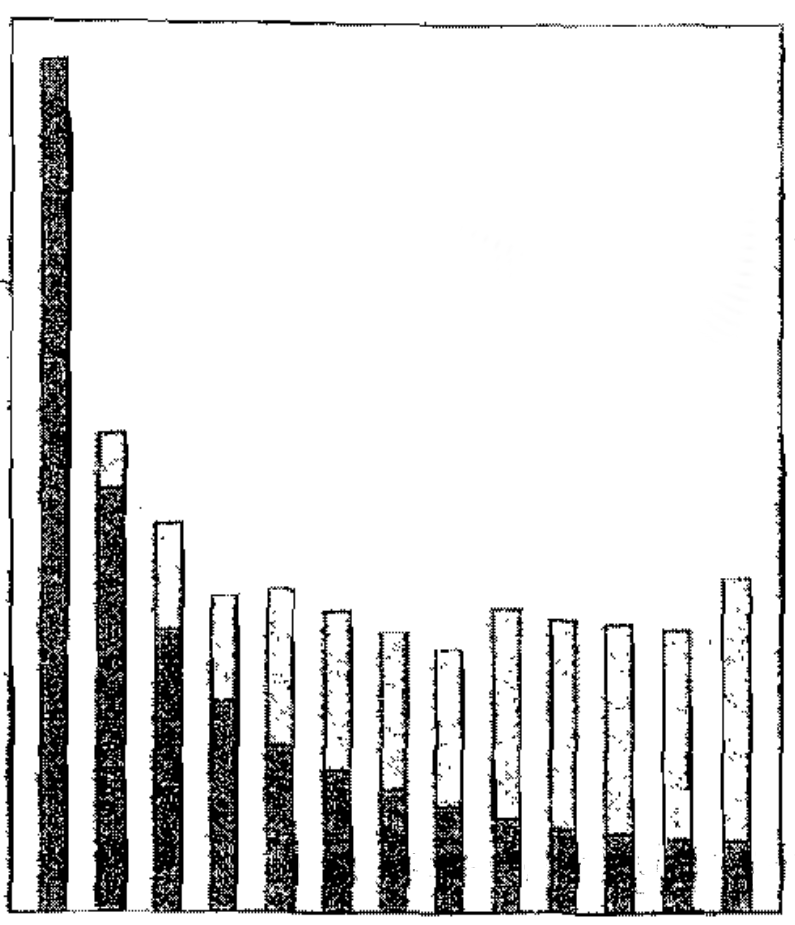
\includegraphics[width=\textwidth]{strong.png}};
        \end{tikzpicture}
        
        {\tiny (d’après M.J. Quinn)}
      \end{center}
    \end{column}
    
    \begin{column}{0.63\textwidth}
      \begin{itemize}
      \item en grisé : temps de calcul
        \begin{itemize}
        \item décroît (ou stagne) lorsque $p \nearrow$
        \end{itemize}

        \medskip
        
      \item en blanc : temps de communication
        \begin{itemize}
        \item augmente lorsque $p \nearrow$
        \end{itemize}

        \medskip
        
      \item Pour un problème donné ($n$ fixé), il existe un nombre maximal de
        processeurs utilisables efficacement
        \begin{itemize}
        \item Au-delà, l'ajout de processeurs supplémentaires n'apporte plus
          de gain de performance
        \end{itemize}
      \end{itemize}
    \end{column}
  \end{columns}  
\end{frame}

%%%%%%%%%%%%%%%%%%%%%%%%%%%%%%%%%%%%%%%%%%%%%%%%%%%%%%%%%%%%%%%%%%%%%

\begin{frame}
\frametitle{Exemple avec un (vrai) programme multi-thread}
\framesubtitle{Calcul de rang de matrices creuses}

\centering
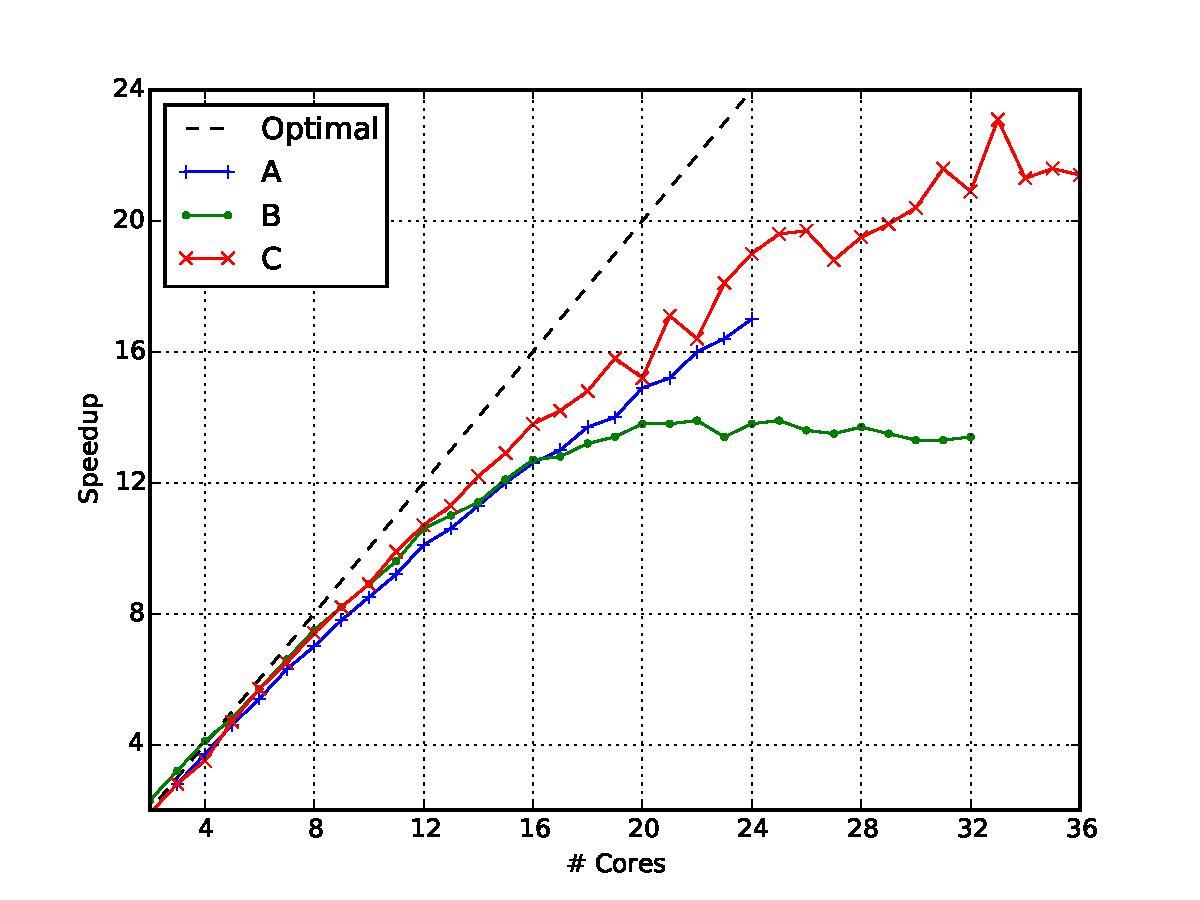
\includegraphics[height=6cm]{d19.pdf}

\medskip

\small
  \begin{tabular}{|c|c|l|c|c|}
\hline
Name & CPU Type        & \# CPU     & cores/CPU & L3 Cache/CPU\\
\hline\hline
A    & Xeon E5-2670 v3 & $2 \times$ & 12        & 30MB\\
\hline
B    & Xeon E5-4620    & $4 \times$ & 8         & 16MB\\
\hline
C    & Xeon E5-2695 v4 & $2 \times$ & 18        & 45MB\\
\hline
\end{tabular}



\end{frame}

%%%%%%%%%%%%%%%%%%%%%%%%%%%%%%%%%%%%%%%%%%%%%%%%%%%%%%%%%%%%%%%%%%%%%

\begin{frame}
\frametitle{Loi d'Amdahl}

Un algorithme dont une fraction $f$ est non
parallélisable. Alors :

\[
  S(n,p)  \leq  \frac{1}{f + (1 - f)/p}
\]

$\Rightarrow$ 20\% d'un algo est séquentiel, l'accélération est 
limitée à 5.

\bigskip

(Sur)co\^ut d\^u au parallélisme \og $1-E(n,p)$ \fg~ 
d\^u aux parties séquentielles et :
\begin{itemize}
\item démarrage et terminaison des tâches 
\item communications et/ou synchronisations  
\item qualité de l'équilibrage de charge (voir cours suivants)
\item surcoûts logiciels dûs aux
  compilateurs, bibliothèques, outils, systèmes d'exploitation... 
\end{itemize}

\end{frame}

%%%%%%%%%%%%%%%%%%%%%%%%%%%%%%%%%%%%%%%%%%%%%%%%%%%%%%%%%%%%%%%%%%%%%
\begin{frame}
\frametitle{\emph{Weak scaling} (\og extensibilité faible \fg)}

\begin{alertblock}{Objectif de la parallélisation}
  \begin{itemize}
  \item Etude des performances quand $n$ augmente avec $p$.
  \item Résoudre de plus gros problèmes en temps fixe.
  \end{itemize}
\end{alertblock}

\medskip

\begin{exampleblock}{Effet d'Amdahl (empirique)}
\begin{itemize}
\item La fraction intrinsèquement séquentielle d'un algo diminue généralement quand $n \nearrow$
\item Coûts de communication $\nearrow$ (car $p \nearrow$), mais \emph{moins
    vite} que la quantité de calculs (car $n \nearrow$).
\end{itemize}
\end{exampleblock}
\end{frame}

%%%%%%%%%%%%%%%%%%%%%%%%%%%%%%%%%%%%%%%%%%%%%%%%%%%%%%%%%%%

\begin{frame}
  \frametitle{Loi de Gustafson-Barsis}

  On exécute un programme parallèle sur $p$ processeurs.

  \medskip
  
  On mesure que la fraction du temps d'exécution passé dans des portions
  intrinsèquement séquentielles est $s$.

  \medskip
  
  Alors :
  \[
    S(n, p)  \leq  p - (p-1)s
  \]

    \medskip
  
    \begin{block}{Exemple}
      Un calcul parallèle s'exécute sur 32 processeurs en 100
      secondes, dont 5 secondes dans des parties séquentielles sur 1 seul
      processeur, alors $ S(n, p)  \leq 30.45$
    \end{block}
  \end{frame}


%%%%%%%%%%%%%%%%%%%%%%%%%%%%%%%%%%%%%%%%%%%%%%%%%%%%%%%%%%%%%%%

\end{document}

% Charles' emacs magic commands
%%% Local Variables:
%%% TeX-engine: xetex
%%% TeX-command-extra: "-shell-escape"
%%% TeX-command-extra-options: "-shell-escape"
%%% ispell-local-dictionary: "english"
%%% eval: (flyspell-mode 1)
%%% eval: (reftex-mode 1)
%%% End:
